\documentclass[10pt]{article}
\usepackage[utf8]{inputenc}
\usepackage[T1]{fontenc}
\usepackage{amsmath}
\usepackage{amsfonts}
\usepackage{amssymb}
\usepackage[version=4]{mhchem}
\usepackage{stmaryrd}
\usepackage{hyperref}
\hypersetup{colorlinks=true, linkcolor=blue, filecolor=magenta, urlcolor=cyan,}
\urlstyle{same}
\usepackage{bbold}
\usepackage{graphicx}
\usepackage[export]{adjustbox}
\graphicspath{ {./images/} }

\title{Multi-Agent Reinforcement Learning: A Selective Overview of Theories and Algorithms }


\author{Kaiqing Zhang ${ }^{\natural} \quad$ Zhuoran Yang ${ }^{\dagger} \quad$ Tamer Başar ${ }^{\natural}$}
\date{}


\begin{document}
\maketitle


\begin{abstract}
Recent years have witnessed significant advances in reinforcement learning (RL), which has registered tremendous success in solving various sequential decision-making problems in machine learning. Most of the successful RL applications, e.g., the games of Go and Poker, robotics, and autonomous driving, involve the participation of more than one single agent, which naturally fall into the realm of multi-agent RL (MARL), a domain with a relatively long history, and has recently re-emerged due to advances in single-agent RL techniques. Though empirically successful, theoretical foundations for MARL are relatively lacking in the literature. In this chapter, we provide a selective overview of MARL, with focus on algorithms backed by theoretical analysis. More specifically, we review the theoretical results of MARL algorithms mainly within two representative frameworks, Markov/stochastic games and extensive-form games, in accordance with the types of tasks they address, i.e., fully cooperative, fully competitive, and a mix of the two. We also introduce several significant but challenging applications of these algorithms. Orthogonal to the existing reviews on MARL, we highlight several new angles and taxonomies of MARL theory, including learning in extensive-form games, decentralized MARL with networked agents, MARL in the mean-field regime, (non-)convergence of policy-based methods for learning in games, etc. Some of the new angles extrapolate from our own research endeavors and interests. Our overall goal with this chapter is, beyond providing an assessment of the current state of the field on the mark, to identify fruitful future research directions on theoretical studies of MARL. We expect this chapter to serve as continuing stimulus for researchers interested in working on this exciting while challenging topic.
\end{abstract}

${ }^{\natural}$ Department of Electrical and Computer Engineering \& Coordinated Science Laboratory, University of Illinois at Urbana-Champaign, 1308 West Main, Urbana, IL, 61801, USA. Email: \{kzhang66, basar1\}@illinois.edu. Writing of this chapter was supported in part by the US Army Research Laboratory (ARL) Cooperative Agreement W911NF-17-2-0196, and in part by the Air Force Office of Scientific Research (AFOSR) Grant FA9550-19-1-0353.

${ }^{\dagger}$ Department of Operations Research and Financial Engineering, Princeton University, 98 Charlton St, Princeton, NJ, 08540, USA. Email: \href{mailto:zy6@princeton.edu}{zy6@princeton.edu}.

\section{Introduction}
Recent years have witnessed sensational advances of reinforcement learning (RL) in many prominent sequential decision-making problems, such as playing the game of Go $[1,2]$, playing real-time strategy games $[3,4]$, robotic control $[5,6]$, playing card games $[7,8]$, and autonomous driving [9], especially accompanied with the development of deep neural networks (DNNs) for function approximation [10]. Intriguingly, most of the successful applications involve the participation of more than one single agent/player ${ }^{1}$, which should be modeled systematically as multi-agent RL (MARL) problems. Specifically, MARL addresses the sequential decision-making problem of multiple autonomous agents that operate in a common environment, each of which aims to optimize its own longterm return by interacting with the environment and other agents [11]. Besides the aforementioned popular ones, learning in multi-agent systems finds potential applications in other subareas, including cyber-physical systems $[12,13]$, finance $[14,15]$, sensor/communication networks $[16,17]$, and social science $[18,19]$.

Largely, MARL algorithms can be placed into three groups, fully cooperative, fully competitive, and a mix of the two, depending on the types of settings they address. In particular, in the cooperative setting, agents collaborate to optimize a common long-term return; while in the competitive setting, the return of agents usually sum up to zero. The mixed setting involves both cooperative and competitive agents, with general-sum returns. Modeling disparate MARL settings requires frameworks spanning from optimization theory, dynamic programming, game theory, and decentralized control, see $\$ 2.2$ for more detailed discussions. In spite of these existing multiple frameworks, several challenges in MARL are in fact common across the different settings, especially for the theoretical analysis. Specifically, first, the learning goals in MARL are multi-dimensional, as the objectives of all agents are not necessarily aligned, which brings up the challenge of dealing with equilibrium points, as well as some additional performance criteria beyond return-optimization, such as the efficiency of communication/coordination, and robustness against potential adversarial agents. Moreover, as all agents are improving their policies according to their own interests concurrently, the environment faced by each agent becomes non-stationary. This breaks or invalidates the basic framework of most theoretical analyses in the single-agent setting. Furthermore, the joint action space that increases exponentially with the number of agents may cause scalability issues, known as the combinatorial nature of MARL [20]. Additionally, the information structure, i.e., who knows what, in MARL is more involved, as each agent has limited access to the observations of others, leading to possibly suboptimal decision rules locally. A detailed elaboration on the underlying challenges can be found in $\S 3$.

There has in fact been no shortage of efforts attempting to address the above challenges. See [11] for a comprehensive overview of earlier theories and algorithms on MARL. Recently, this domain has gained resurgence of interest due to the advances of

${ }^{1}$ Hereafter, we will use agent and player interchangeably. single-agent RL techniques. Indeed, a huge volume of work on MARL has appeared lately, focusing on either identifying new learning criteria and/or setups [21, 22, 23, 24], or developing new algorithms for existing setups, thanks to the development of deep learning $[25,26,27,28,29,30,31]$, operations research [32, 33, 34, 35], and multi-agent systems [36, 37, 38, 39]. Nevertheless, not all the efforts are placed under rigorous theoretical footings, partly due to the limited understanding of even single-agent deep RL theories, and partly due to the inherent challenges in multi-agent settings. As a consequence, it is imperative to review and organize the MARL algorithms with theoretical guarantees, in order to highlight the boundary of existing research endeavors, and stimulate potential future directions on this topic.

In this chapter, we provide a selective overview of theories and algorithms in MARL, together with several significant while challenging applications. More specifically, we focus on two representative frameworks of MARL, namely, Markov/stochastic games and extensive-form games, in discrete-time settings as in standard single-agent RL. In conformity with the aforementioned three groups, we review and pay particular attention to MARL algorithms with convergence and complexity analysis, most of which are fairly recent. With this focus in mind, we note that our overview is by no means comprehensive. In fact, besides the classical reference [11], there are several other reviews on MARL that have appeared recently, due to the resurgence of MARL [40, 20, 41, 42]. We would like to emphasize that these reviews provide views and taxonomies that are complementary to ours: [40] surveys the works that are specifically devised to address opponent-induced non-stationarity, one of the challenges we discuss in $\S 3 ;[20,41]$ are relatively more comprehensive, but with the focal point on deep MARL, a subarea with scarce theories thus far; [42], on the other hand, focuses on algorithms in the cooperative setting only, though the review within this setting is extensive.

Finally, we spotlight several new angles and taxonomies that are comparatively underexplored in the existing MARL reviews, primarily owing to our own research endeavors and interests. First, we discuss the framework of extensive-form games in MARL, in addition to the conventional one of Markov games, or even simplified repeated games $[11,40,20]$; second, we summarize the progresses of a recently boosting subarea: decentralized MARL with networked agents, as an extrapolation of our early works on this $[23,43,44]$; third, we bring about the mean-field regime into MARL, as a remedy for the case with an extremely large population of agents; fourth, we highlight some recent advances in optimization theory, which shed lights on the (non-)convergence of policy-based methods for MARL, especially zero-sum games. We have also reviewed some of the literature on MARL in partially observed settings, but without using deep RL as heuristic solutions. We expect these new angles to help identify fruitful future research directions, and more importantly, inspire researchers with interests in establishing rigorous theoretical foundations on MARL.

Roadmap. The remainder of this chapter is organized as follows. In $\S 2$, we introduce the background of MARL: standard algorithms for single-agent RL, and the frameworks of MARL. In §3, we summarize several challenges in developing MARL theory, in addition to the single-agent counterparts. A series of MARL algorithms, mostly with theoretical guarantees, are reviewed and organized in $\S 4$, according to the types of tasks they address. In $\S 5$, we briefly introduce a few recent successes of MARL driven by the algorithms mentioned, followed by conclusions and several open research directions outlined in $\S 6$.

\section{Background}
In this section, we provide the necessary background on reinforcement learning, in both single- and multi-agent settings.

\subsection{Single-Agent RL}
A reinforcement learning agent is modeled to perform sequential decision-making by interacting with the environment. The environment is usually formulated as an infinitehorizon discounted Markov decision process (MDP), henceforth referred to as Markov decision process ${ }^{2}$, which is formally defined as follows.

Definition 2.1 A Markov decision process is defined by a tuple $(\mathcal{S}, \mathcal{A}, \mathcal{P}, R, \gamma)$, where $\mathcal{S}$ and $\mathcal{A}$ denote the state and action spaces, respectively; $\mathcal{P}: \mathcal{S} \times \mathcal{A} \rightarrow \Delta(\mathcal{S})$ denotes the transition probability from any state $s \in \mathcal{S}$ to any state $s^{\prime} \in \mathcal{S}$ for any given action $a \in \mathcal{A} ; R: \mathcal{S} \times \mathcal{A} \times \mathcal{S} \rightarrow$ $\mathbb{R}$ is the reward function that determines the immediate reward received by the agent for a transition from $(s, a)$ to $s^{\prime} ; \gamma \in[0,1)$ is the discount factor that trades off the instantaneous and future rewards.

As a standard model, MDP has been widely adopted to characterize the decisionmaking of an agent with full observability of the system state $s .{ }^{3}$ At each time $t$, the agent chooses to execute an action $a_{t}$ in face of the system state $s_{t}$, which causes the system to transition to $s_{t+1} \sim \mathcal{P}\left(\cdot \mid s_{t}, a_{t}\right)$. Moreover, the agent receives an instantaneous reward $R\left(s_{t}, a_{t}, s_{t+1}\right)$. The goal of solving the MDP is thus to find a policy $\pi: \mathcal{S} \rightarrow \Delta(\mathcal{A})$, a mapping from the state space $\mathcal{S}$ to the distribution over the action space $\mathcal{A}$, so that $a_{t} \sim \pi\left(\cdot \mid s_{t}\right)$ and the discounted accumulated reward

\[
\mathbb{E}\left[\sum_{t \geq 0} \gamma^{t} R\left(s_{t}, a_{t}, s_{t+1}\right) \mid a_{t} \sim \pi\left(\cdot \mid s_{t}\right), s_{0}\right]
\]

${ }^{2}$ Note that there are several other standard formulations of MDPs, e.g., time-average-reward setting and finite-horizon episodic setting. Here, we only present the classical infinite-horizon discounted setting for ease of exposition.

${ }^{3}$ The partially observed MDP (POMDP) model is usually advocated when the agent has no access to the exact system state but only an observation of the state. See $[45,46]$ for more details on the POMDP model. is maximized. Accordingly, one can define the action-value function (Q-function) and state-value function (V-function) under policy $\pi$ as

\[
\begin{aligned}
Q_{\pi}(s, a) & =\mathbb{E}\left[\sum_{t \geq 0} \gamma^{t} R\left(s_{t}, a_{t}, s_{t+1}\right) \mid a_{t} \sim \pi\left(\cdot \mid s_{t}\right), a_{0}=a, s_{0}=s\right], \\
V_{\pi}(s) & =\mathbb{E}\left[\sum_{t \geq 0} \gamma^{t} R\left(s_{t}, a_{t}, s_{t+1}\right) \mid a_{t} \sim \pi\left(\cdot \mid s_{t}\right), s_{0}=s\right]
\end{aligned}
\]

for any $s \in \mathcal{S}$ and $a \in \mathcal{A}$, which are the discounted accumulated reward starting from $\left(s_{0}, a_{0}\right)=(s, a)$ and $s_{0}=s$, respectively. The ones corresponding to the optimal policy $\pi^{*}$ are usually referred to as the optimal $Q$-function and the optimal state-value function, respectively.

By virtue of the Markovian property, the optimal policy can be obtained by dynamicprogramming/backward induction approaches, e.g., value iteration and policy iteration algorithms [47], which require the knowledge of the model, i.e., the transition probability and the form of reward function. Reinforcement learning, on the other hand, is to find such an optimal policy without knowing the model. The RL agent learns the policy from experiences collected by interacting with the environment. By and large, RL algorithms can be categorized into two mainstream types, value-based and policy-based methods.

\subsubsection{Value-Based Methods}
Value-based RL methods are devised to find a good estimate of the state-action value function, namely, the optimal Q-function $Q_{\pi^{*}}$. The (approximate) optimal policy can then be extracted by taking the greedy action of the Q-function estimate. One of the most popular value-based algorithms is Q-learning [48], where the agent maintains an estimate of the Q-value function $\hat{Q}(s, a)$. When transitioning from state-action pair $(s, a)$ to next state $s^{\prime}$, the agent receives a payoff $r$ and updates the Q-function according to:

\[
\hat{Q}(s, a) \leftarrow(1-\alpha) \hat{Q}(s, a)+\alpha\left[r+\gamma \max _{a^{\prime}} \hat{Q}\left(s^{\prime}, a^{\prime}\right)\right],
\]

where $\alpha>0$ is the stepsize/learning rate. Under certain conditions on $\alpha, \mathrm{Q}$-learning can be proved to converge to the optimal Q-value function almost surely [48, 49], with finite state and action spaces. Moreover, when combined with neural networks for function approximation, deep Q-learning has achieved great empirical breakthroughs in humanlevel control applications [10]. Another popular on-policy value-based method is SARSA, whose convergence was established in [50] for finite-space settings.

An alternative while popular value-based RL algorithm is Monte-Carlo tree search (MCTS) $[51,52,53]$, which estimates the optimal value function by constructing a search tree via Monte-Carlo simulations. Tree polices that judiciously select actions to balance exploration-exploitation are used to build and update the search tree. The most common tree policy is to apply the UCB1 (UCB stands for upper confidence bound) algorithm, which was originally devised for stochastic multi-arm bandit problems $[54,55]$, to each node of the tree. This yields the popular UCT algorithm [52]. Recent research endeavors on the non-asymptotic convergence of MCTS include [56, 57].

Besides, another significant task regarding value functions in RL is to estimate the value function associated with a given policy (not only the optimal one). This task, usually referred to as policy evaluation, has been tackled by algorithms that follow a similar update as (2.1), named temporal difference (TD) learning $[58,59,60]$. Some other common policy evaluation algorithms with convergence guarantees include gradient TD methods with linear [61, 62, 63], and nonlinear function approximations [64]. See [65] for a more detailed review on policy evaluation.

\subsubsection{Policy-Based Methods}
Another type of RL algorithms directly searches over the policy space, which is usually estimated by parameterized function approximators like neural networks, namely, approximating $\pi(\cdot \mid s) \approx \pi_{\theta}(\cdot \mid s)$. As a consequence, the most straightforward idea, which is to update the parameter along the gradient direction of the long-term reward, has been instantiated by the policy gradient (PG) method. As a key premise for the idea, the closedform of $P G$ is given as [66]

\[
\nabla J(\theta)=\mathbb{E}_{a \sim \pi_{\theta}(\cdot \mid s), s \sim \eta_{\pi_{\theta}}(\cdot)}\left[Q_{\pi_{\theta}}(s, a) \nabla \log \pi_{\theta}(a \mid s)\right],
\]

where $J(\theta)$ and $Q_{\pi_{\theta}}$ are the expected return and Q-function under policy $\pi_{\theta}$, respectively, $\nabla \log \pi_{\theta}(a \mid s)$ is the score function of the policy, and $\eta_{\pi_{\theta}}$ is the state occupancy measure, either discounted or ergodic, under policy $\pi_{\theta}$. Then, various policy gradient methods, including REINFORCE [67], G(PO)MDP [68], and actor-critic algorithms [69, 70], have been proposed by estimating the gradient in different ways. A similar idea also applies to deterministic policies in continuous-action settings, whose PG form has been derived recently by [71]. Besides gradient-based ones, several other policy optimization methods have achieved state-of-the-art performance in many applications, including PPO [72], TRPO [73], soft actor-critic [74].

Compared with value-based RL methods, policy-based ones enjoy better convergence guarantees $[69,75,76,77]$, especially with neural networks for function approximation $[78,79]$, which can readily handle massive or even continuous state-action spaces. Besides the value- and policy-based methods, there also exist RL algorithms based on the linear program formulation of an MDP; see recent efforts in [80,81].

\subsection{Multi-Agent RL Framework}
In a similar vein, multi-agent RL also addresses sequential decision-making problems, but with more than one agent involved. In particular, both the evolution of the system

\begin{center}
\includegraphics[max width=\textwidth]{2023_07_26_beef0e26e91281a60b0cg-07(1)}
\end{center}

(a) Markov decision process

\begin{center}
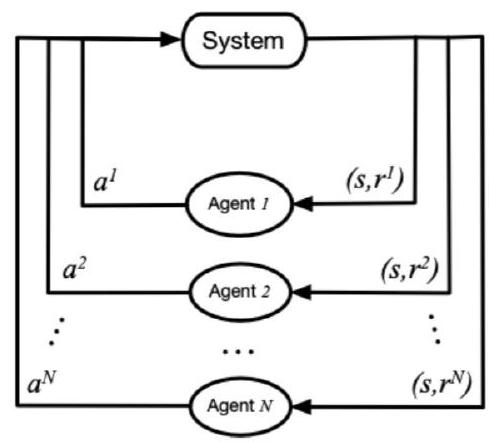
\includegraphics[max width=\textwidth]{2023_07_26_beef0e26e91281a60b0cg-07}
\end{center}

(b) Markov game

\begin{center}
\includegraphics[max width=\textwidth]{2023_07_26_beef0e26e91281a60b0cg-07(2)}
\end{center}

(c) Extensive-form game

Figure 1: Schematic diagrams for the system evolution of a Markov decision process, a Markov game, and an extensive-form game, which correspond to the frameworks for single- and multi-agent RL, respectively. Specifically, in an MDP as in (a), the agent observes the state $s$ and receives reward $r$ from the system, after outputting the action $a$; in an MG as in (b), all agents choose actions $a^{i}$ simultaneously, after observing the system state $s$ and receiving each individual reward $r^{i}$; in a two-player extensive-form game as in (c), the agents make decisions on choosing actions $a^{i}$ alternately, and receive each individual reward $r^{i}(z)$ at the end of the game, with $z$ being the terminal history. In the imperfect information case, player 2 is uncertain about where he/she is in the game, which makes the information set non-singleton.

state and the reward received by each agent are influenced by the joint actions of all agents. More intriguingly, each agent has its own long-term reward to optimize, which now becomes a function of the policies of all other agents. Such a general model finds broad applications in practice, see $\$ 5$ for a detailed review of several prominent examples.

In general, there exist two seemingly different but closely related theoretical frameworks for MARL, Markov/stochastic games and extensive-form games, as to be introduced next. Evolution of the systems under different frameworks are illustrated in Figure 1.

\subsubsection{Markov/Stochastic Games}
One direct generalization of MDP that captures the intertwinement of multiple agents is Markov games (MGs), also known as stochastic games [82]. Originated from the seminal work [83], the framework of $\mathrm{MGs}^{4}$ has long been used in the literature to develop MARL algorithms, see $\S 4$ for more details. We introduce the formal definition as below.

Definition 2.2 A Markov game is defined by a tuple $\left(\mathcal{N}, \mathcal{S},\left\{\mathcal{A}^{i}\right\}_{i \in \mathcal{N}}, \mathcal{P},\left\{R^{i}\right\}_{i \in \mathcal{N}}, \gamma\right)$, where $\mathcal{N}=\{1, \cdots, N\}$ denotes the set of $N>1$ agents, $\mathcal{S}$ denotes the state space observed by all agents, $\mathcal{A}^{i}$ denotes the action space of agent $i$. Let $\mathcal{A}:=\mathcal{A}^{1} \times \cdots \times \mathcal{A}^{N}$, then $\mathcal{P}: \mathcal{S} \times \mathcal{A} \rightarrow \Delta(\mathcal{S})$ denotes

${ }^{4}$ Similar to the single-agent setting, here we only introduce the infinite-horizon discounted setting for simplicity, though other settings of MGs, e.g., time-average-reward setting and finite-horizon episodic setting, also exist [84]. the transition probability from any state $s \in \mathcal{S}$ to any state $s^{\prime} \in \mathcal{S}$ for any joint action $a \in \mathcal{A}$; $R^{i}: \mathcal{S} \times \mathcal{A} \times \mathcal{S} \rightarrow \mathbb{R}$ is the reward function that determines the immediate reward received by agent $i$ for a transition from $(s, a)$ to $s^{\prime} ; \gamma \in[0,1)$ is the discount factor.

At time $t$, each agent $i \in \mathcal{N}$ executes an action $a_{t}^{i}$, according to the system state $s_{t}$. The system then transitions to state $s_{t+1}$, and rewards each agent $i$ by $R^{i}\left(s_{t}, a_{t}, s_{t+1}\right)$. The goal of agent $i$ is to optimize its own long-term reward, by finding the policy $\pi^{i}: \mathcal{S} \rightarrow \Delta\left(\mathcal{A}^{i}\right)$ such that $a_{t}^{i} \sim \pi^{i}\left(\cdot \mid s_{t}\right)$. As a consequence, the value-function $V^{i}: \mathcal{S} \rightarrow \mathbb{R}$ of agent $i$ becomes a function of the joint policy $\pi: \mathcal{S} \rightarrow \Delta(\mathcal{A})$ defined as $\pi(a \mid s):=\prod_{i \in \mathcal{N}} \pi^{i}\left(a^{i} \mid s\right)$. In particular, for any joint policy $\pi$ and state $s \in \mathcal{S}$,

\[
V_{\pi^{i}, \pi^{-i}}^{i}(s):=\mathbb{E}\left[\sum_{t \geq 0} \gamma^{t} R^{i}\left(s_{t}, a_{t}, s_{t+1}\right) \mid a_{t}^{i} \sim \pi^{i}\left(\cdot \mid s_{t}\right), s_{0}=s\right],
\]

where $-i$ represents the indices of all agents in $\mathcal{N}$ except agent $i$. Hence, the solution concept of an MG deviates from that of an MDP, since the optimal performance of each agent is controlled not only by its own policy, but also the choices of all other players of the game. The most common solution concept, Nash equilibrium (NE) $)^{5}$, is defined as follows $[85,84]$.

Definition 2.3 A Nash equilibrium of the Markov game $\left(\mathcal{N}, \mathcal{S},\left\{\mathcal{A}^{i}\right\}_{i \in \mathcal{N}}, \mathcal{P},\left\{R^{i}\right\}_{i \in \mathcal{N}}, \gamma\right)$ is a joint policy $\pi^{*}=\left(\pi^{1, *}, \cdots, \pi^{N, *}\right)$, such that for any $s \in \mathcal{S}$ and $i \in \mathcal{N}$

\[
V_{\pi^{i, *}, \pi^{-i, *}}^{i}(s) \geq V_{\pi^{i}, \pi^{-i, *}}^{i}(s), \quad \text { for any } \pi^{i}
\]

Nash equilibrium characterizes an equilibrium point $\pi^{*}$, from which none of the agents has any incentive to deviate. In other words, for any agent $i \in \mathcal{N}$, the policy $\pi^{i, *}$ is the bestresponse of $\pi^{-i, *}$. As a standard learning goal for MARL, NE always exists for finite-space infinite-horizon discounted MGs [84], but may not be unique in general. Most of the MARL algorithms are contrived to converge to such an equilibrium point, if it exists.

The framework of Markov games is general enough to umbrella various MARL settings summarized below.

\section{Cooperative Setting:}
In a fully cooperative setting, all agents usually share a common reward function, i.e., $R^{1}=R^{2}=\cdots=R^{N}=R$. We note that this model is also referred to as multi-agent MDPs (MMDPs) in the AI community [86, 87], and Markov teams/team Markov games in the control/game theory community [88, 89, 90, 91]. Moreover, from the game-theoretic perspective, this cooperative setting can also be viewed as a special case of Markov potential games [92, 22, 93], with the potential function being the common accumulated

${ }^{5}$ Here, we focus only on stationary Markov Nash equilibria, for the infinite-horizon discounted MGs considered. reward. With this model in mind, the value function and Q-function are identical to all agents, which thus enables the single-agent RL algorithms, e.g., Q-learning update (2.1), to be applied, if all agents are coordinated as one decision maker. The global optimum for cooperation now constitutes a Nash equilibrium of the game.

Besides the common-reward model, another slightly more general and surging model for cooperative MARL considers team-average reward [94, 23, 95]. Specifically, agents are allowed to have different reward functions, which may be kept private to each agent, while the goal for cooperation is to optimize the long-term reward corresponding to the average reward $\bar{R}\left(s, a, s^{\prime}\right):=N^{-1} \cdot \sum_{i \in \mathcal{N}} R^{i}\left(s, a, s^{\prime}\right)$ for any $\left(s, a, s^{\prime}\right) \in \mathcal{S} \times \mathcal{A} \times \mathcal{S}$. The averagereward model, which allows more heterogeneity among agents, includes the model above as a special case. It also preserves privacy among agents, and facilitates the development of decentralized MARL algorithms $[94,23,96]$. Such heterogeneity also necessitates the incorporation of communication protocols into MARL, and the analysis of communicationefficient MARL algorithms.

\section{Competitive Setting:}
Fully competitive setting in MARL is typically modeled as zero-sum Markov games, namely, $\sum_{i \in \mathcal{N}} R^{i}\left(s, a, s^{\prime}\right)=0$ for any $\left(s, a, s^{\prime}\right)$. For ease of algorithm analysis and computational tractability, most literature focused on two agents that compete against each other [83], where clearly the reward of one agent is exactly the loss of the other. In addition to direct applications to game-playing $[83,2,97]$, zero-sum games also serve as a model for robust learning, since the uncertainty that impedes the learning process of the agent can be accounted for as a fictitious opponent in the game that is always against the agent $[98,99,100]$. Therefore, the Nash equilibrium yields a robust policy that optimizes the worst-case long-term reward.

\section{Mixed Setting:}
Mixed setting is also known as the general-sum game setting, where no restriction is imposed on the goal and relationship among agents [101, 102]. Each agent is selfinterested, whose reward may be conflicting with others'. Equilibrium solution concepts from game theory, such as Nash equilibrium [85], have the most significant influence on algorithms that are developed for this general setting. Furthermore, we include the setting with both fully cooperative and competitive agents, for example, two zero-sum competitive teams with cooperative agents in each team $[103,44,3]$, as instances of the mixed setting as well.

\subsubsection{Extensive-Form Games}
Even though they constitute a classical formalism for MARL, Markov games can only handle the fully observed case, i.e., the agent has perfect information on the system state $s_{t}$ and the executed action $a_{t}$ at time $t$. Nonetheless, a plethora of MARL applications involve agents with only partial observability, i.e., imperfect information of the game. Ex- tension of Markov games to partially observed case may be applicable, which, however, is challenging to solve, even under the cooperative setting $[36,104]{ }^{6}$

In contrast, another framework, named extensive-form games [105, 106], can handily model imperfect information for multi-agent decision-making. This framework is rooted in computational game theory and has been shown to admit polynomial-time algorithms under mild conditions [107]. We briefly introduce the framework of extensiveform games as follows.

Definition 2.4 An extensive-form game is defined by $\left(\mathcal{N} \cup\{c\}, \mathcal{H}, \mathcal{Z}, \mathcal{A},\left\{R^{i}\right\}_{i \in \mathcal{N}}, \tau, \pi^{c}, \mathcal{S}\right)$, where $\mathcal{N}=\{1, \ldots, N\}$ denotes the set of $N>1$ agents, and $c$ is a special agent called chance or nature, which has a fixed stochastic policy that specifies the randomness of the environment. Besides, $\mathcal{A}$ is the set of all possible actions that agents can take and $\mathcal{H}$ is the set of all possible histories, where each history is a sequence of actions taken from the beginning of the game. Let $\mathcal{A}(h)=\{a \mid h a \in \mathcal{H}\}$ denote the set of actions available after a nonterminal history $h$. Suppose an agent takes action $a \in \mathcal{A}(h)$ given history $h \in \mathcal{H}$, which then leads to a new history ha $\in \mathcal{H}$. Among all histories, $\mathcal{Z} \subseteq \mathcal{H}$ is a subset of terminal histories that represents the completion of a game. A utility is assigned to each agent $i \in \mathcal{N}$ at a terminal history, dictated by the function $R^{i}: \mathcal{Z} \rightarrow \mathbb{R}$. Moreover, $\tau: \mathcal{H} \rightarrow \mathcal{N} \cup\{c\}$ is the identification function that specifies which agent takes the action at each history. If $\tau(h)=c$, the chance agent takes an action a according to its policy $\pi^{c}$, i.e., $a \sim \pi^{c}(\cdot \mid h)$. Furthermore, $\mathcal{S}$ is the partition of $\mathcal{H}$ such that for any $s \in \mathcal{S}$ and any $h, h^{\prime} \in s$, we have $\tau(h)=\tau\left(h^{\prime}\right)$ and $\mathcal{A}(h)=\mathcal{A}\left(h^{\prime}\right)$. In other words, histories $h$ and $h^{\prime}$ in the same partition are indistinguishable to the agent that is about to take action, namely $\tau(h)$. The elements in $\mathcal{S}$ are referred to as information states.

Intuitively, the imperfect information of an extensive-form game is reflected by the fact that agents cannot distinguish between histories in the same information set. Since we have $\tau(h)=\tau\left(h^{\prime}\right)$ and $\mathcal{A}(h)=\mathcal{A}\left(h^{\prime}\right)$ for all $h, h^{\prime} \in s$ and $s \in \mathcal{S}$, for ease of presentation, in the sequel, for all $h \in s$, we let $\mathcal{A}(s)$ and $\tau(s)$ denote $\mathcal{A}(h)$ and $\tau(h)$, respectively. We also define a mapping $I: \mathcal{H} \rightarrow \mathcal{S}$ by letting $I(h)=s$ if $h \in s$. Moreover, we only consider games where both $\mathcal{H}$ and $\mathcal{A}$ are finite sets. To simplify the notation, for any two histories $h, h^{\prime} \in \mathcal{H}$, we refer to $h$ as a prefix of $h^{\prime}$, denoted by $h \sqsubseteq h^{\prime}$, if $h^{\prime}$ can be reached from $h$ by taking a sequence of actions. In this case, we call $h^{\prime}$ a suffix of $h$. Furthermore, we assume throughout that the game features perfect recall, which implies that each agent remembers the sequence of the information states and actions that have led to its current information state. The assumption of perfect recall is commonly made in the literature, which enables the existence of polynomial-time algorithms for solving the game [107]. More importantly, by the celebrated Kuhn's theorem [108], under such an assumption, to find the set of Nash equilibria, it suffices to restrict the derivation to the set of behavioral policies which map each information set $s \in \mathcal{S}$ to a probability distribution over $\mathcal{A}(s)$. For

${ }^{6}$ Partially observed Markov games under the cooperative setting are usually formulated as decentralized POMDP (Dec-POMDP) problems. See $§ 4.1 .3$ for more discussions on this setting. any $i \in \mathcal{N}$, let $\mathcal{S}^{i}=\{s \in \mathcal{S}: \tau(s)=i\}$ be the set of information states of agent $i$. A joint policy of the agents is denoted by $\pi=\left(\pi^{1}, \ldots, \pi^{N}\right)$, where $\pi^{i}: \mathcal{S}^{i} \rightarrow \Delta(\mathcal{A}(s))$ is the policy of agent $i$. For any history $h$ and any joint policy $\pi$, we define the reach probability of $h$ under $\pi$ as

\[
\eta_{\pi}(h)=\prod_{h^{\prime}: h^{\prime} a \sqsubseteq h} \pi^{\tau\left(h^{\prime}\right)}\left(a \mid I\left(h^{\prime}\right)\right)=\prod_{i \in \mathcal{N} \cup\{c\}} \prod_{h^{\prime}: h^{\prime} a \sqsubseteq h, \tau\left(h^{\prime}\right)=i} \pi^{i}\left(a \mid I\left(h^{\prime}\right)\right),
\]

which specifies the probability that $h$ is created when all agents follow $\pi$. We similarly define the reach probability of an information state $s$ under $\pi$ as $\eta_{\pi}(s)=\sum_{h \in s} \eta_{\pi}(h)$. The expected utility of agent $i \in \mathcal{N}$ is thus given by $\sum_{z \in \mathcal{Z}} \eta_{\pi}(z) \cdot R^{i}(z)$, which is denoted by $R^{i}(\pi)$ for simplicity. Now we are ready to introduce the solution concept for extensiveform games, i.e., Nash equilibrium and its $\epsilon$-approximation, as follows.

Definition 2.5 An $\epsilon$-Nash equilibrium of an extensive-form game represented by $(\mathcal{N} \cup\{c\}, \mathcal{H}, \mathcal{Z}$, $\left.\mathcal{A},\left\{R^{i}\right\}_{i \in \mathcal{N}}, \tau, \pi^{c}, \mathcal{S}\right)$ is a joint policy $\pi^{*}=\left(\pi^{1, *}, \cdots, \pi^{N, *}\right)$, such that for any $i \in \mathcal{N}$,

\[
R^{i}\left(\pi^{i, *}, \pi^{-i, *}\right) \geq R^{i}\left(\pi^{i}, \pi^{-i, *}\right)-\epsilon, \quad \text { for any policy } \pi^{i} \text { of agent } i .
\]

Here $\pi^{-i}$ denotes the joint policy of agents in $\mathcal{N} \backslash\{i\}$ where agent $j$ adopts policy $\pi^{j}$ for all $j \in \mathcal{N} \backslash\{i\}$. Additionally, if $\epsilon=0, \pi^{*}$ constitutes a Nash equilibrium.

\section{Various Settings:}
Extensive-form games are in general used to model non-cooperative settings. Specifically, zero-sum/constant-sum utility with $\sum_{i \in \mathcal{N}} R^{i}=k$ for some constant $k$ corresponds to the fully competitive setting; general-sum utility function results in the mixed setting. More importantly, settings of different information structures can also be characterized by extensive-form games. In particular, a perfect information game is one where each information set is a singleton, i.e., for any $s \in \mathcal{S},|s|=1$; an imperfect information game is one where there exists $s \in \mathcal{S},|s|>1$. In other words, with imperfect information, the information state $s$ used for decision-making represents more than one possible history, and the agent cannot distinguish between them.

Among various settings, the zero-sum imperfect information setting has been the main focus of theoretical studies that bridge MARL and extensive-form games $[109,110,111$, 112]. It has also motivated MARL algorithms that revolutionized competitive setting applications like Poker AI [113, 8].

\section{Connection to Markov Games:}
Note that the two formalisms in Definitions 2.2 and 2.4 are connected. In particular, for simultaneous-move Markov games, the choices of actions by other agents are unknown to an agent, which thus leads to different histories that can be aggregated as one information state $s$. Histories in these games are then sequences of joint actions, and the discounted accumulated reward instantiates the utility at the end of the game. Conversely, by simply setting $\mathcal{A}^{j}=\emptyset$ at the state $s$ for agents $j \neq \tau(s)$, the extensive-form game reduces to a Markov game with state-dependent action spaces. See [114] for a more detailed discussion on the connection.

Remark 2.6 (Other MARL Frameworks) Several other theoretical frameworks for MARL also exist in the literature, e.g., normal-form and/or repeated games $[115,116,117,118]$, and partially observed Markov games [119, 120, 121]. However, the former framework can be viewed as a special case of MGs, with a singleton state; most early theories of MARL in this framework have been restricted to small scale problems $[116,118,117]$ only. MARL in the latter framework, on the other hand, is inherently challenging to address in general [104, 119], leading to relatively scarce theories in the literature. Due to space limitation, we do not introduce these models here in any detail. We will briefly review MARL algorithms under some of these models, especially the partially observed setting, in $\S 4$, though. Interested readers are referred to the early review [11] for more discussions on MARL in normal-form/repeated games.

\section{Challenges in MARL Theory}
Despite a general model that finds broad applications, MARL suffers from several challenges in theoretical analysis, in addition to those that arise in single-agent RL. We summarize below the challenges that we regard as fundamental in developing theories for MARL.

\subsection{Non-Unique Learning Goals}
Unlike single-agent RL, where the goal of the agent is to maximize the long-term return efficiently, the learning goals of MARL can be vague at times. In fact, as argued in [122], the unclarity of the problems being addressed is the fundamental flaw in many early MARL works. Indeed, the goals that need to be considered in the analysis of MARL algorithms can be multi-dimensional. The most common goal, which has, however, been challenged in [122], is the convergence to Nash equilibrium as defined in §2.2. By definition, NE characterizes the point that no agent will deviate from, if any algorithm finally converges. This is undoubtedly a reasonable solution concept in game theory, under the assumption that the agents are all rational, and are capable of perfectly reasoning and infinite mutual modeling of agents. However, with bounded rationality, the agents may only be able to perform finite mutual modeling [106]. As a result, the learning dynamics that are devised to converge to NE may not be justifiable for practical MARL agents. Instead, the goal may be focused on designing the best learning strategy for a given agent and a fixed class of the other agents in the game. In fact, these two goals are styled as equilibrium agenda and AI agenda in [122]. Besides, it has also been controversial that convergence (to the equilibrium point) is the dominant performance criterion for MARL algorithm analysis. In fact, it has been recognized in [123] that value-based MARL algorithms fail to converge to the stationary NE of general-sum Markov games, which motivated the new solution concept of cyclic equilibrium therein, at which the agents cycle rigidly through a set of stationary policies, i.e., not converging to any NE policy. Alternatively, $[116,124]$ separate the learning goal into being both stable and rational, where the former ensures the algorithm to be convergent, given a predefined, targeted class of opponents' algorithms, while the latter requires the convergence to a best-response when the other agents remain stationary. If all agents are both stable and rational, convergence to NE naturally arises in this context. Moreover, the notion of regret introduces another angle to capture agents' rationality, which measures the performance of the algorithm compared to the best hindsight static strategy $[116,125,126]$. No-regret algorithms with asymptotically zero average regret guarantee the convergence to the equilibria of certain games $[127,125,109]$, which in essence guarantee that the agent is not exploited by others.

In addition to the goals concerning optimizing the return, several other goals that are special to multi-agent systems have also drawn increasing attention. For example, [128, 21,129 ] investigate learning to communicate, in order for the agents to better coordinate. Such a concern on communication protocols has naturally inspired the recent studies on communication-efficient MARL [130, 131, 132, 133]. Other important goals include how to learn without over-fitting certain agents $[134,26,135]$, and how to learn robustly with either malicious/adversarial or failed/dysfunctional learning agents [136, 137, 138]. Still in their infancy, some works concerning aforementioned goals provide only empirical results, leaving plenty of room for theoretical studies.

\subsection{Non-Stationarity}
Another key challenge of MARL lies in the fact that multiple agents usually learn concurrently, causing the environment faced by each individual agent to be non-stationary. In particular, the action taken by one agent affects the reward of other opponent agents, and the evolution of the state. As a result, the learning agent is required to account for how the other agents behave and adapt to the joint behavior accordingly. This invalidates the stationarity assumption for establishing the convergence of single-agent RL algorithms, namely, the stationary Markovian property of the environment such that the individual reward and current state depend only on the previous state and action taken. This precludes the direct use of mathematical tools for single-agent RL analysis in MARL.

Indeed, theoretically, if the agent ignores this issue and optimizes its own policy assuming a stationary environment, which is usually referred to as an independent learner, the algorithms may fail to converge $[139,115]$, except for several special settings $[37,38]$. Empirically, however, independent learning may achieve satisfiable performance in practice $[140,141]$. As the most well-known issue in MARL, non-stationarity has long been recognized in the literature $[11,142]$. A recent comprehensive survey [40] peculiarly provides an overview on how it is modeled and addressed by state-of-the-art multi-agent learning algorithms. We thus do not include any further discussion on this challenge, and refer interested readers to [40].

\subsection{Scalability Issue}
To handle non-stationarity, each individual agent may need to account for the joint action space, whose dimension increases exponentially with the number of agents. This is also referred to as the combinatorial nature of MARL [20]. Having a large number of agents complicates the theoretical analysis, especially the convergence analysis, of MARL. This argument is substantiated by the fact that theories on MARL for the two-player zero-sum setting are much more extensive and advanced than those for general-sum settings with more than two agents, see $\S 4$ for a detailed comparison. One possible remedy for the scalability issue is to assume additionally the factorized structures of either the value or reward functions with regard to the action dependence; see [143, 144, 145] for the original heuristic ideas, and $[146,147]$ for recent empirical progress. Relevant theoretical analysis had not been established until recently [148], which considers a special dependence structure, and develops a provably convergent model-based algorithm.

Another theoretical challenge of MARL that is brought about independently of, but worsened by, the scalability issue, is to build up theories for deep multi-agent RL. Particularly, scalability issues necessitate the use of function approximation, especially deep neural networks, in MARL. Though empirically successful, the theoretical analysis of deep MARL is an almost uncharted territory, with the currently limited understanding of deep learning theory, not alone the deep RL theory. This is included as one of the future research directions in $\S 6$.

\subsection{Various Information Structures}
Compared to the single-agent case, the information structure of MARL, namely, who knows what at the training and execution, is more involved. For example, in the framework of Markov games, it suffices to observe the instantaneous state $s_{t}$, in order for each agent to make decisions, since the local policy $\pi^{i}$ mapping from $\mathcal{S}$ to $\Delta\left(\mathcal{A}^{i}\right)$ contains the equilibrium policy. On the other hand, for extensive-form games, each agent may need to recall the history of past decisions, under the common perfect recall assumption. Furthermore, as self-interested agents, each agent can scarcely access either the policy or the rewards of the opponents, but at most the action samples taken by them. This partial information aggravates the issues caused by non-stationarity, as the samples can hardly recover the exact behavior of the opponents' underlying policies, which increases the non-stationarity viewed by individual agents. The extreme case is the aforementioned independent learning scheme, which assumes the observability of only the local action and

\begin{center}
\includegraphics[max width=\textwidth]{2023_07_26_beef0e26e91281a60b0cg-15}
\end{center}

(a) Centralized setting

\begin{center}
\includegraphics[max width=\textwidth]{2023_07_26_beef0e26e91281a60b0cg-15(2)}
\end{center}

(b) Decentralized setting with networked agents

\begin{center}
\includegraphics[max width=\textwidth]{2023_07_26_beef0e26e91281a60b0cg-15(1)}
\end{center}

(c) Fully decentralized setting

Figure 2: Three representative information structures in MARL. Specifically, in (a), there exists a central controller that can aggregate information from the agents, e.g., joint actions, joint rewards, and joint observations, and even design policies for all agents. The information exchanged between the central controller and the agents can thus include both some private observations from the agents, and the local policies designed for each agent from the controller. In both (b) and (c), there is no such a central controller, and are thus both referred to as decentralized structures. In (b), agents are connected via a possibly time-varying communication network, so that the local information can spread across the network, by information exchange with only each agent's neighbors. (b) is more common in cooperative MARL settings. In (c), the agents are full decentralized, with no explicit information exchange with each other. Instead, each agent makes decisions based on its local observations, without any coordination and/or aggregation of data. The local observations that vary across agents, however, may contain some global information, e.g., the joint actions of other agents, namely the control sharing information structure [149]. Such a fully decentralized structure can also be found in many game-theoretic learning algorithms.

reward, and suffers from non-convergence in general [139].

Learning schemes resulting from various information structures lead to various levels of difficulty for theoretical analysis. Specifically, to mitigate the partial information issue above, a great deal of work assumes the existence of a central controller that can collect information such as joint actions, joint rewards, and joint observations, and even design policies for all agents [119, 150, 26, 141, 28, 151, 152, 130, 147]. This structure gives birth to the popular learning scheme of centralized-learning-decentralized-execution, which stemmed from the works on planning for the partially observed setting, namely, Dec-POMDPs $[119,150,153]$, and has been widely adopted in recent (deep) MARL works $[26,141,28,151,130,147]$. For cooperative settings, this learning scheme greatly simplifies the analysis, allowing the use of tools for single-agent RL analysis. Though, for non-cooperative settings with heterogeneous agents, this scheme does not significantly simplify the analysis, as the learning goals of the agents are not aligned, see §3.1.

Nonetheless, generally such a central controller does not exist in many applications, except the ones that can easily access a simulator, such as video games and robotics. As a consequence, a fully decentralized learning scheme is preferred, which includes the aforementioned independent learning scheme as a special case. To address the nonconvergence issue in independent learning, agents are usually allowed to exchange/share local information with their neighbors over a communication network [94, 154, 155, 23, $43,44,156,96,95,157,158,131]$. We refer to this setting as a decentralized one with networked agents. Theoretical analysis for convergence is then made possible in this setting, the difficulty of which sits between that of single-agent RL and general MARL algorithms. Three different information structures are depicted in Figure 2.

\section{MARL Algorithms with Theory}
This section provides a selective review of MARL algorithms, and categorizes them according to the tasks to address. Exclusively, we review here the works that are focused on the theoretical studies only, which are mostly built upon the two representative MARL frameworks, fully observed Markov games and extensive-form games, introduced in §2.2. A brief summary on MARL for partially observed Markov games in cooperative settings, namely, the Dec-POMDP problems, is also provided below in $\S 4.1$, due to their relatively more mature theory than that of MARL for general partially observed Markov games.

\subsection{Cooperative Setting}
Cooperative MARL constitutes a great portion of MARL settings, where all agents collaborate with each other to achieve some shared goal. Most cooperative MARL algorithms backed by theoretical analysis are devised for the following more specific settings.

\subsubsection{Homogeneous Agents}
A majority of cooperative MARL settings involve homogeneous agents with a common reward function that aligns all agents' interests. In the extreme case with large populations of agents, such a homogeneity also indicates that the agents play an interchangeable role in the system evolution, and can hardly be distinguished from each other. We elaborate more on homogeneity below.

\section{Multi-Agent MDP \& Markov Teams}
Consider a Markov game as in Definition 2.2 with $R^{1}=R^{2}=\cdots=R^{N}=R$, where the reward $R: \mathcal{S} \times \mathcal{A} \times \mathcal{S} \rightarrow \mathbb{R}$ is influenced by the joint action in $\mathcal{A}=\mathcal{A}^{1} \times \cdots \times \mathcal{A}^{N}$. As a result, the $\mathrm{Q}$-function is identical for all agents. Hence, a straightforward algorithm proceeds by performing the standard Q-learning update (2.1) at each agent, but taking the max over the joint action space $a^{\prime} \in \mathcal{A}$. Convergence to the optimal/equilibrium $\mathrm{Q}$-function has been established in $[49,159]$, when both state and action spaces are finite. However, convergence of the Q-function does not necessarily imply that of the equilibrium policy for the Markov team, as any combination of equilibrium policies extracted at each agent may not constitute an equilibrium policy, if the equilibrium policies are nonunique, and the agents fail to agree on which one to select. Hence, convergence to the NE policy is only guaranteed if either the equilibrium is assumed to be unique [159], or the agents are coordinated for equilibrium selection. The latter idea has first been validated in the cooperative repeated games setting [115], a special case of Markov teams with a singleton state, where the agents are joint-action learners (JAL), maintaining a Q-value for joint actions, and learning empirical models of all others. Convergence to equilibrium point is claimed in [115], without a formal proof. For the actual Markov teams, this coordination has been exploited in [90], which proposes optimal adaptive learning (OAL), the first MARL algorithm with provable convergence to the equilibrium policy. Specifically, OAL first learns the game structure, and constructs virtual games at each state that are weakly acyclic with respect to (w.r.t.) a biased set. OAL can be shown to converge to the NE, by introducing the biased adaptive play learning algorithm for the constructed weakly acyclic games, motivated from [160].

Apart from equilibrium selection, another subtlety special to Markov teams (compared to single-agent RL) is the necessity to address the scalability issue, see §3.3. As independent Q-learning may fail to converge [139], one early attempt toward developing scalable while convergent algorithms for MMDPs is [87], which advocates a distributed Q-learning algorithm that converges for deterministic finite MMDPs. Each agent maintains only a Q-table of state $s$ and local action $a^{i}$, and successively takes maximization over the joint action $a^{\prime}$. No other agent's actions and their histories can be acquired by each individual agent. Several other heuristics (with no theoretical backing) regarding either reward or value function factorization have been proposed to mitigate the scalability issue [143, 144, 145, 146, 147]. Very recently, [161] provides a rigorous characterization of conditions that justify this value factorization idea. Another recent theoretical work along this direction is [148], which imposes a special dependence structure, i.e., a one-directional tree, so that the (near-)optimal policy of the overall MMDP can be provably well-approximated by local policies. More recently, [38] has studied common interest games, which includes Markov teams as an example, and develops a decentralized RL algorithm that relies on only states, local actions and rewards. With the same information structure as independent Q-learning [139], the algorithm is guaranteed to converge to team optimal equilibrium policies, and not just equilibrium policies. This is important as in general, a suboptimal equilibrium can perform arbitrarily worse than the optimal equilibrium [38].

For policy-based methods, to our knowledge, the only convergence guarantee for this setting exists in [162]. The authors propose two-timescale actor-critic fictitious play algorithms, where at the slower timescale, the actor mixes the current policy and the bestresponse one w.r.t. the local Q-value estimate, while at the faster timescale the critic performs policy evaluation, as if all agents' policies are stationary. Convergence is estab- lished for simultaneous move multistage games with a common (also zero-sum, see §4.2.2) reward, a special Markov team with initial and absorbing states, and each state being visited only once.

\section{Markov Potential Games}
From a game-theoretic perspective, a more general framework to embrace cooperation is potential games [163], where there exits some potential function shared by all agents, such that if any agent changes its policy unilaterally, the change in its reward equals (or proportions to) that in the potential function. Though most potential games are stateless, an extension named Markov potential games (MPGs) has gained increasing attention for modeling sequential decision-making [92, 22], which includes Markovian states whose evolution is affected by the joint actions. Indeed, MMDPs/Markov teams constitute a particular case of MPGs, with the potential function being the common reward; such dynamic games can also be viewed as being strategically equivalent to Markov teams, using the terminology in, e.g., [164, Chapter 1]. Under this model, [93] provides verifiable conditions for a Markov game to be an MPG, and shows the equivalence between finding closed-loop NE in MPG and solving a single-agent optimal control problem. Hence, single-agent RL algorithms are then enabled to solve this MARL problem.

\section{Mean-Field Regime}
Another idea toward tackling the scalability issue is to take the setting to the meanfield regime, with an extremely large number of homogeneous agents. Each agent's effect on the overall multi-agent system can thus become infinitesimal, resulting in all agents being interchangeable/indistinguishable. The interaction with other agents, however, is captured simply by some mean-field quantity, e.g., the average state, or the empirical distribution of states. Each agent only needs to find the best response to the mean-field, which considerably simplifies the analysis. This mean-field view of multi-agent systems has been approached by the mean-field games (MFGs) model [165, 166, 167, 168, 169], the team model with mean-field sharing $[170,171]$, and the game model with mean-field actions [172]. ${ }^{7}$

MARL in these models have not been explored until recently, mostly in the noncooperative setting of MFGs, see $\S 4.3$ for a more detailed review. Regarding the cooperative setting, recent work [175] studies RL for Markov teams with mean-field sharing $[170,176,171]$. Compared to MFG, the model considers agents that share a common reward function depending only on the local state and the mean-field, which encourages cooperation among the agents. Also, the term mean-field refers to the empirical average for the states of finite population, in contrast to the expectation and probability distribution of infinite population in MFGs. Based on the dynamic programming decomposition for the

${ }^{7}$ The difference between mean-field teams and mean-field games is mainly the solution concept: optimum versus equilibrium, as the difference between general dynamic team theory $[173,88,174]$ and game theory $[82,84]$. Although the former can be viewed as a special case of the latter, related works are usually reviewed separately in the literature. We follow here this convention. specified model [170], several popular RL algorithms are easily translated to address this setting [175]. More recently, $[177,178]$ approach the problem from a mean-field control (MFC) model, to model large-population of cooperative decision-makers. Policy gradient methods are proved to converge for linear quadratic MFCs in [177], and mean-field Q-learning is then shown to converge for general MFCs [178].

\subsubsection{Decentralized Paradigm with Networked Agents}
Cooperative agents in numerous practical multi-agent systems are not always homogeneous. Agents may have different preferences, i.e., reward functions, while they still form a team to maximize the return of the team-average reward $\bar{R}$, with $\bar{R}\left(s, a, s^{\prime}\right)=N^{-1}$. $\sum_{i \in \mathcal{N}} R^{i}\left(s, a, s^{\prime}\right)$. More subtly, the reward function is sometimes not sharable with others, as the preference is kept private to each agent. This setting finds broad applications in engineering systems as sensor networks [179], smart grid [180, 181], intelligent transportation systems $[12,182]$, and robotics [183].

Covering the homogeneous setting in $\S 4.1 .1$ as a special case, the specified one definitely requires more coordination, as, for example, the global value function cannot be estimated locally without knowing other agents' reward functions. With a central controller, most MARL algorithms reviewed in §4.1.1 directly apply, since the controller can collect and average the rewards, and distributes the information to all agents. Nonetheless, such a controller may not exist in most aforementioned applications, due to either cost, scalability, or robustness concerns $[179,180,184]$. Instead, the agents may be able to share/exchange information with their neighbors over a possibly time-varying and sparse communication network, as illustrated in Figure 2 (b). Though MARL under this decentralized/distributed ${ }^{8}$ paradigm is imperative, it is relatively less-investigated, in comparison to the extensive results on distributed/consensus algorithms that solve static/one-stage optimization problems $[185,186,187,188]$, which, unlike RL, involves no system dynamics, and does not maximize the long-term objective as a sequential-decision making problem.

\section{Learning Optimal Policy}
The most significant goal is to learn the optimal joint policy, while each agent only accesses to local and neighboring information over the network. The idea of MARL with networked agents dates back to [189]. To our knowledge, the first provably convergent MARL algorithm under this setting is due to [94], which incorporates the idea of consensus + innovation to the standard Q-learning algorithm, yielding the $\mathcal{Q D}$-learning algorithm

${ }^{8}$ Note that hereafter we use decentralized and distributed interchangeably for describing this paradigm. with the following update

\[
\begin{gathered}
Q_{t+1}^{i}(s, a) \leftarrow Q_{t}^{i}(s, a)+\alpha_{t, s, a}\left[R^{i}(s, a)+\gamma \max _{a^{\prime} \in \mathcal{A}} Q_{t}^{i}\left(s^{\prime}, a^{\prime}\right)-Q_{t}^{i}(s, a)\right] \\
-\beta_{t, s, a} \sum_{j \in \mathcal{N}_{t}^{i}}\left[Q_{t}^{i}(s, a)-Q_{t}^{j}(s, a)\right],
\end{gathered}
\]

where $\alpha_{t, s, a}, \beta_{t, s, a}>0$ are stepsizes, $\mathcal{N}_{t}^{i}$ denotes the set of neighboring agents of agent $i$, at time $t$. Compared to the Q-learning update (2.1), $\mathcal{Q} \mathcal{D}$-learning appends an innovation term that captures the difference of Q-value estimates from its neighbors. With certain conditions on the stepsizes, the algorithm is guaranteed to converge to the optimum Qfunction for the tabular setting.

Due to the scalability issue, function approximation is vital in MARL, which necessitates the development of policy-based algorithms. Our work [23] proposes actorcritic algorithms for this setting. Particularly, each agent parameterizes its own policy $\pi_{\theta^{i}}^{i}: \mathcal{S} \rightarrow \Delta\left(\mathcal{A}^{i}\right)$ by some parameter $\theta^{i} \in \mathbb{R}^{m^{i}}$, the policy gradient of the return is first derived as

\[
\nabla_{\theta^{i}} J(\theta)=\mathbb{E}\left[\nabla_{\theta^{i}} \log \pi_{\theta^{i}}^{i}\left(s, a^{i}\right) \cdot Q_{\theta}(s, a)\right]
\]

where $Q_{\theta}$ is the global value function corresponding to $\bar{R}$ under the joint policy $\pi_{\theta}$ that is defined as $\pi_{\theta}(a \mid s):=\prod_{i \in \mathcal{N}} \pi_{\theta^{i}}^{i}\left(a^{i} \mid s\right)$. As an analogy to (2.2), the policy gradient in (4.1) involves the expectation of the product between the local score function $\nabla_{\theta^{i}} \log \pi_{\theta^{i}}^{i}\left(s, a^{i}\right)$ and the global Q-function $Q_{\theta}$. The latter, nonetheless, cannot be estimated individually at each agent. As a result, by parameterizing each local copy of $Q_{\theta}(\cdot, \cdot)$ as $Q_{\theta}\left(\cdot, \cdot ; \omega^{i}\right)$ for agent $i$, we propose the following consensus-based TD learning for the critic step, i.e., for estimating $Q_{\theta}(\cdot, \cdot)$ :

\[
\widetilde{\omega}_{t}^{i}=\omega_{t}^{i}+\beta_{\omega, t} \cdot \delta_{t}^{i} \cdot \nabla_{\omega} Q_{t}\left(\omega_{t}^{i}\right), \quad \quad \omega_{t+1}^{i}=\sum_{j \in \mathcal{N}} c_{t}(i, j) \cdot \widetilde{\omega}_{t}^{j},
\]

where $\beta_{\omega, t}>0$ is the stepsize, $\delta_{t}^{i}$ is the local TD-error calculated using $Q_{\theta}\left(\cdot, \cdot ; \omega^{i}\right)$. The first relation in (4.2) performs the standard TD update, followed by a weighted combination of the neighbors' estimates $\widetilde{\omega}_{t}^{j}$. The weights here, $c_{t}(i, j)$, are dictated by the topology of the communication network, with non-zero values only if two agents $i$ and $j$ are connected at time $t$. They also need to satisfy the doubly stochastic property in expectation, so that $\omega_{t}^{i}$ reaches a consensual value for all $i \in \mathcal{N}$ if it converges. Then, each agent $i$ updates its policy following stochastic policy gradient given by (4.1) in the actor step, using its own Q-function estimate $Q_{\theta}\left(\cdot, \cdot ; \omega_{t}^{i}\right)$. A variant algorithm is also introduced in [23], relying on not the Q-function, but the state-value function approximation, to estimate the global advantage function. With these in mind, almost sure convergence is established in [23] for these decentralized actor-critic algorithms, when linear functions are used for value function approximation. Similar ideas are also extended to the setting with continuous spaces [43], where deterministic policy gradient (DPG) method is usually used. Off-policy exploration, namely a stochastic behavior policy, is required for DPG, as the deterministic on-policy may not be explorative enough. However, in the multi-agent setting, as the policies of other agents are unknown, the common off-policy approach for DPG [71, §4.2] does not apply. Inspired by the expected policy gradient (EPG) method [190] which unifies stochastic PG (SPG) and DPG, we develop an algorithm that remains on-policy, but reduces the variance of general SPG [43]. In particular, we derive the multi-agent version of EPG, based on which we develop the actor step that can be implemented in a decentralized fashion, while the critic step still follows (4.2). Convergence of the algorithm is then also established when linear function approximation is used [43]. In the same vein, [158] considers the extension of [23] to an off-policy setting, building upon the emphatic temporal differences (ETD) method for the critic [191]. By incorporating the analysis of $\operatorname{ETD}(\lambda)$ [192] into [23], almost sure convergence guarantee has also been established. Another off-policy algorithm for the same setting is proposed concurrently by [193], where agents do not share their estimates of value function. Instead, the agents aim to reach consensus over the global optimal policy estimation. Provable convergence is then established for the algorithm, with a local critic and a consensus actor.

RL for decentralized networked agents has also been investigated in multi-task, in addition to the multi-agent, settings. In some sense, the former can be regarded as a simplified version of the latter, where each agent deals with an independent MDP that is not affected by other agents, while the goal is still to learn the optimal joint policy that accounts for the average reward of all agents. [194] proposes a distributed actor-critic algorithm, assuming that the states, actions, and rewards are all local to each agent. Each agent performs a local TD-based critic step, followed by a consensus-based actor step that follows the gradient calculated using information exchanged from the neighbors. Gradient of the average return is then proved to converge to zero as the iteration goes to infinity. [155] has developed Diff-DAC, another distributed actor-critic algorithm for this setting, from duality theory. The updates resemble those in [23], but provide additional insights that actor-critic is actually an instance of the dual ascent method for solving a linear program.

Note that all the aforementioned convergence guarantees are asymptotic, i.e., the algorithms converge as the iteration numbers go to infinity, and are restricted to the case with linear function approximations. This fails to quantify the performance when finite iterations and/or samples are used, not to mention when nonlinear functions such as deep neural networks are utilized. As an initial step toward finite-sample analyses in this setting with more general function approximation, we consider in [44] the batch RL algorithms [195], specifically, decentralized variants of the fitted-Q iteration (FQI) [196, 197]. Note that we focus on FQI since it motivates the celebrated deep Q-learning algorithm [10] when deep neural networks are used for function approximation. We study FQI variants for both the cooperative setting with networked agents, and the competitive setting with two teams of such networked agents (see $§ 4.2 .1$ for more details). In the former setting, all agents cooperate to iteratively update the global Q-function estimate, by fitting nonlinear least squares with the target values as the responses. In particular, let $\mathcal{F}$ be the function class for Q-function approximation, $\left\{\left(s_{j},\left\{a_{j}^{i}\right\}_{i \in \mathcal{N}}, s_{j}^{\prime}\right)\right\}_{j \in[n]}$ be the batch transitions dataset of size $n$ available to all agents, $\left\{r_{j}^{i}\right\}_{j \in[n]}$ be the local reward samples private to each agent, and $y_{j}^{i}=r_{j}^{i}+\gamma \cdot \max _{a \in \mathcal{A}} Q_{t}^{i}\left(s_{j}^{\prime}, a\right)$ be the local target value, where $Q_{t}^{i}$ is agent $i$ 's Q-function estimate at iteration $t$. Then, all agents cooperate to find a common Q-function estimate by solving

\[
\min _{f \in \mathcal{F}} \frac{1}{N} \sum_{i \in \mathcal{N}} \frac{1}{2 n} \sum_{j=1}^{n}\left[y_{j}^{i}-f\left(s_{j}, a_{j}^{1}, \cdots, a_{j}^{N}\right)\right]^{2} .
\]

Since $y_{j}^{i}$ is only known to agent $i$, the problem in (4.3) aligns with the formulation of distributed/consensus optimization in [185, 186, 187, 188, 198, 199], whose global optimal solution can be achieved by the algorithms therein, if $\mathcal{F}$ makes $\sum_{j=1}^{n}\left[y_{j}^{i}-f\left(s_{j}, a_{j}^{1}, \cdots, a_{j}^{N}\right)\right]^{2}$ convex for each $i$. This is indeed the case if $\mathcal{F}$ is a linear function class. Nevertheless, with only a finite iteration of distributed optimization algorithms (common in practice), agents may not reach exact consensus, leading to an error of each agent's Q-function estimate away from the actual optimum of (4.3). Such an error also exists when nonlinear function approximation is used. Considering this error caused by decentralized computation, we follow the error propagation analysis stemming from single-agent batch RL [200, 201, 197, 202, 203], to establish the finite-sample performance of the proposed algorithms, i.e., how the accuracy of the algorithms output depends on the function class $\mathcal{F}$, the number of samples within each iteration $n$, and the number of iterations $t$.

\section{Policy Evaluation}
Aside from control, a series of algorithms in this setting focuses on the policy evaluation task only, namely, the critic step of the actor-critic algorithms. With the policy fixed, this task embraces a neater formulation, as the sampling distribution becomes stationary, and the objective becomes convex under linear function approximation. This facilitates the finite-time/sample analyses, in contrast to most control algorithms with only asymptotic guarantees. Specifically, under joint policy $\pi$, suppose each agent parameterizes the value function by a linear function class $\left\{V_{\omega}(s):=\phi^{\top}(s) \omega: \omega \in \mathbb{R}^{d}\right\}$, where $\phi(s) \in \mathbb{R}^{d}$ is the feature vector at $s \in \mathcal{S}$, and $\omega \in \mathbb{R}^{d}$ is the vector of parameters. For notational convenience, let $\Phi:=\left(\cdots ; \phi^{\top}(s) ; \cdots\right) \in \mathbb{R}^{|\mathcal{S}| \times d}, D=\operatorname{diag}\left[\left\{\eta_{\pi}(s)\right\}_{s \in \mathcal{S}}\right] \in \mathbb{R}^{|\mathcal{S}| \times|\mathcal{S}|}$ be a diagonal matrix constructed using the state-occupancy measure $\eta_{\pi}, \bar{R}^{\pi}(s)=N^{-1} \cdot \sum_{i \in \mathcal{N}} R^{i, \pi}(s)$, where $R^{i, \pi}(s)=\mathbb{E}_{a \sim \pi(\cdot \mid s), s^{\prime} \sim P(\cdot \mid s, a)}\left[R^{i}\left(s, a, s^{\prime}\right)\right]$, and $P^{\pi} \in \mathbb{R}^{|\mathcal{S}| \times|\mathcal{S}|}$ with the $\left(s, s^{\prime}\right)$ element being $\left[P^{\pi}\right]_{s, s^{\prime}}=\sum_{a \in \mathcal{A}} \pi(a \mid s) P\left(s^{\prime} \mid s, a\right)$. Then, the objective of all agents is to jointly minimize the mean square projected Bellman error (MSPBE) associated with the team-average reward, i.e.,

\[
\min _{\omega} \operatorname{MSPBE}(\omega):=\left\|\Pi_{\Phi}\left(V_{\omega}-\gamma P^{\pi} V_{\omega}-\bar{R}^{\pi}\right)\right\|_{D}^{2}=\|A \omega-b\|_{C^{-1}}^{2}
\]

where $\Pi_{\Phi}: \mathbb{R}^{|\mathcal{S}|} \rightarrow \mathbb{R}^{|\mathcal{S}|}$ defined as $\Pi_{\Phi}:=\Phi\left(\Phi^{\top} D \Phi\right)^{-1} \Phi^{\top} D$ is the projection operator onto subspace $\left\{\Phi \omega: \omega \in \mathbb{R}^{d}\right\}, A:=\mathbb{E}\left\{\phi(s)\left[\phi(s)-\gamma \phi\left(s^{\prime}\right)\right]^{\top}\right\}, C:=\mathbb{E}\left[\phi(s) \phi^{\top}(s)\right]$, and $b:=$ $\mathbb{E}\left[\bar{R}^{\pi}(s) \phi(s)\right]$. By replacing the expectation with samples and using the Fenchel duality, the finite-sum version of (4.4) can be re-formulated as a distributed saddle-point problem

\[
\min _{\omega} \max _{\lambda^{i}, i \in \mathcal{N}} \frac{1}{N n} \sum_{i \in \mathcal{N}} \sum_{j=1}^{n} 2\left(\lambda^{i}\right)^{\top} A_{j} \omega-2\left(b_{j}^{i}\right)^{\top} \lambda^{i}-\left(\lambda^{i}\right)^{\top} C_{j} \lambda^{i}
\]

where $n$ is the data size, $A_{j}, C_{j}$ and $b_{j}^{i}$ are empirical estimates of $A, C$ and $b^{i}:=\mathbb{E}\left[R^{i, \pi}(s) \phi(s)\right]$, respectively, using sample $j$. Note that (4.5) is convex in $\omega$ and concave in $\left\{\lambda^{i}\right\}_{i \in \mathcal{N}}$. The use of MSPBE as an objective is standard in multi-agent policy evaluation [154, 156, 96, 95, 157], and the idea of saddle-point reformulation has been adopted in [154, 156, 96, 204]. Note that in [204], a variant of MSPBE, named H-truncated $\lambda$-weighted MSPBE, is advocated, in order to control the bias of the solution deviated from the actual mean square Bellman error minimizer.

With the formulation (4.4) in mind, [156] develops a distributed variant of the gradient TD-based method, with asymptotic convergence established using the ordinary differential equation (ODE) method. In [96], a double averaging scheme that combines the dynamic consensus [205] and the SAG algorithm [206] has been proposed to solve the saddle-point problem (4.5) with a linear rate. [204] incorporates the idea of variancereduction, specifically, AVRG in [207], into gradient TD-based policy evaluation. Achieving the same linear rate as [96], three advantages are claimed in [204]: i) data-independent memory requirement; ii) use of eligibility traces [208]; iii) no need for synchronization in sampling. More recently, standard TD learning [58], instead of gradient-TD, has been generalized to this MARL setting, with special focuses on finite-sample analyses $[95,157]$. Distributed TD(0) is first studied in [95], using the proof techniques originated in [209], which requires a projection on the iterates, and the data samples to be independent and identically distributed (i.i.d.). Furthermore, motivated by the recent progress in [210], finite-time performance of the more general distributed $\operatorname{TD}(\lambda)$ algorithm is provided in [157], with neither projection nor i.i.d. noise assumption needed.

Policy evaluation for networked agents has also been investigated under the setting of independent agents interacting with independent MDPs. [154] studies off-policy evaluation based on the importance sampling technique. With no coupling among MDPs, an agent does not need to know the actions of the other agents. Diffusion-based distributed GTD is then proposed, and is shown to convergence in the mean-square sense with a sublinear rate. In [211], two variants of the TD-learning, namely, GTD2 and TDC [62], have been designed for this setting, with weak convergence proved by the general stochastic approximation theory in [212], when agents are connected by a time-varying communication network. Note that [204] also considers the independent MDP setting, with the same results established as the actual MARL setting.

\section{Other Learning Goals}
Several other learning goals have also been explored for decentralized MARL with networked agents. [213] has considered the optimal consensus problem, where each agent over the network tracks the states of its neighbors' as well as a leader's, so that the consensus error is minimized by the joint policy. A policy iteration algorithm is then introduced, followed by a practical actor-critic algorithm using neural networks for function approximation. A similar consensus error objective is also adopted in [214], under the name of cooperative multi-agent graphical games. A centralized-critic-decentralized-actor scheme is utilized for developing off-policy RL algorithms.

Communication efficiency, as a key ingredient in the algorithm design for this setting, has drawn increasing attention recently [130, 132, 131]. Specifically, [130] develops Lazily Aggregated Policy Gradient (LAPG), a distributed PG algorithm that can reduce the communication rounds between the agents and a central controller, by judiciously designing communication trigger rules. [132] addresses the same policy evaluation problem as [96], and develops a hierarchical distributed algorithm by proposing a mixing matrix different from the doubly stochastic one used in $[23,96,156]$, which allows unidirectional information exchange among agents to save communication. In contrast, the distributed actor-critic algorithm in [131] reduces the communication by transmitting only one scalar entry of its state vector at each iteration, while preserving provable convergence as in [23].

\subsubsection{Partially Observed Model}
We complete the overview for cooperative settings by briefly introducing a class of significant but challenging models where agents are faced with partial observability. Though common in practice, theoretical analysis of MARL algorithms in this setting is still relatively scarce, in contrast to the aforementioned fully observed settings. In general, this setting can be modeled by a decentralized POMDP (Dec-POMDP) [36], which shares almost all elements such as the reward function and the transition model, as the MMDP/Markov team model in $\$ 2.2 .1$, except that each agent now only has its local observations of the system state $s$. With no accessibility to other agents' observations, an individual agent cannot maintain a global belief state, the sufficient statistic for decision making in single-agent POMDPs. Hence, Dec-POMDPs have been known to be NEXP-complete [104], requiring super-exponential time to solve in the worst case.

There is an increasing interest in developing planning/learning algorithms for DecPOMDPs. Most of the algorithms are based on the centralized-learning-decentralized-execution scheme. In particular, the decentralized problem is first reformulated as a centralized one, which can be solved at a central controller with (a simulator that generates) the ob- servation data of all agents. The policies are then optimized/learned using data, and distributed to all agents for execution. Finite-state controllers (FSCs) are commonly used to represent the local policy at each agent $[215,216]$, which map local observation histories to actions. A Bayesian nonparametric approach is proposed in [217] to determine the controller size of variable-size FSCs. To efficiently solve the centralized problem, a series of top-down algorithms have been proposed. In [150], the Dec-POMDP is converted to nonobservable MDP (NOMDP), a kind of centralized sequential decision-making problem, which is then addressed by some heuristic tree search algorithms. As an extension of the NOMDP conversion, $[218,152]$ convert Dec-POMDPs to occupancy-state MDPs (oMDPs), where the occupancy-states are distributions over hidden states and joint histories of observations. As the value functions of oMDPs enjoy the piece-wise linearity and convexity, both tractable planning [218] and value-based learning [152] algorithms have been developed.

To further improve computational efficiency, several sampling-based planning/learning algorithms have also been proposed. In particular, Monte-Carlo sampling with policy iteration and the expectation-maximization algorithm, are proposed in [219] and [220], respectively. Furthermore, Monte-Carlo tree search has been applied to special classes of Dec-POMDPs, such as multi-agent POMDPs [121] and multi-robot active perception [221]. In addition, policy gradient-based algorithms can also be developed for this centralized learning scheme [152], with a centralized critic and a decentralized actor. Finitesample analysis can also be established under this scheme $[222,223]$, for tabular settings with finite state-action spaces.

Several attempts have also been made to enable decentralized learning in Dec-POMDPs. When the agents share some common information/observations, [224] proposes to reformulate the problem as a centralized POMDP, with the common information being the observations of a virtual central controller. This way, the centralized POMDP can be solved individually by each agent. In [225], the reformulated POMDP has been approximated by finite-state MDPs with exponentially decreasing approximation error, which are then solved by Q-learning. Very recently, [39] has developed a tree-search based algorithm for solving this centralized POMDP, which, interestingly, echoes back the heuristics for solving Dec-POMDPs directly as in $[121,221]$, but with a more solid theoretical footing. Note that in both $[225,39]$, a common random number generator is used for all agents, in order to avoid communication among agents and enable a decentralized learning scheme.

\subsection{Competitive Setting}
Competitive settings are usually modeled as zero-sum games. Computationally, there exists a great barrier between solving two-player and multi-player zero-sum games. In particular, even the simplest three-player matrix games, are known to be PPAD-complete $[226,227]$. Thus, most existing results on competitive MARL focus on two-player zerosum games, with $\mathcal{N}=\{1,2\}$ and $R^{1}+R^{2}=0$ in Definitions 2.2 and 2.4. In the rest of this section, we review methods that provably find a Nash (equivalently, saddle-point) equilibrium in two-player Markov or extensive-form games. The existing algorithms can mainly be categorized into two classes: value-based and policy-based approaches, which are introduced separately in the sequel.

\subsubsection{Value-Based Methods}
Similar as in single-agent MDPs, value-based methods aim to find an optimal value function from which the joint Nash equilibrium policy can be extracted. Moreover, the optimal value function is known to be the unique fixed point of a Bellman operator, which can be obtained via dynamic programming type methods.

Specifically, for simultaneous-move Markov games, the value function defined in (2.3) satisfies $V_{\pi^{1}, \pi^{2}}^{1}=-V_{\pi^{1}, \pi^{2}}^{2}$. and thus any Nash equilibrium $\pi^{*}=\left(\pi^{1, *}, \pi^{2, *}\right)$ satisfies

\[
V_{\pi^{1}, \pi^{1, *}}^{1}(s) \leq V_{\pi^{1, *}, \pi^{2, *}}^{1}(s) \leq V_{\pi^{1, *}, \pi^{2}}^{1}(s), \quad \text { for any } \pi=\left(\pi^{1}, \pi^{2}\right) \text { and } s \in \mathcal{S} .
\]

Similar as the minimax theorem in normal-form/matrix zero-sum games [228], for twoplayer zero-sum Markov games with finite state and action spaces, one can define the optimal value function $V^{*}: \mathcal{S} \rightarrow \mathbb{R}$ as

\[
V^{*}=\max _{\pi^{1}} \min _{\pi^{2}} V_{\pi^{1}, \pi^{2}}^{1}=\min _{\pi^{2}} \max _{\pi^{1}} V_{\pi^{1}, \pi^{2}}^{1}
\]

Then (4.6) implies that $V_{\pi^{1, *}, \pi^{2, *}}^{1}$ coincides with $V^{*}$ and any pair of policies $\pi^{1}$ and $\pi^{2}$ that attains the supremum and infimum in (4.7) constitutes a Nash equilibrium. Moreover, similar to MDPs, [82] shows that $V^{*}$ is the unique solution of a Bellman equation and a Nash equilibrium can be constructed based on $V^{*}$. Specifically, for any $V: \mathcal{S} \rightarrow \mathbb{R}$ and any $s \in \mathcal{S}$, we define

\[
Q_{V}\left(s, a^{1}, a^{2}\right)=\mathbb{E}_{s^{\prime} \sim \mathcal{P}\left(\cdot \mid s, a^{1}, a^{2}\right)}\left[R^{1}\left(s, a^{1}, a^{2}, s^{\prime}\right)+\gamma \cdot V\left(s^{\prime}\right)\right]
\]

where $Q_{V}(s, \cdot, \cdot)$ can be regarded as a matrix in $\mathbb{R}^{\left|\mathcal{A}^{1}\right| \times\left|\mathcal{A}^{2}\right|}$. Then we define the Bellman operator $\mathcal{T}^{*}$ by solving a matrix zero-sum game regarding $Q_{V}(s, \cdot, \cdot)$ as the payoff matrix, i.e., for any $s \in \mathcal{S}$, one can define

\[
\left(\mathcal{T}^{*} V\right)(s)=\operatorname{Value}\left[Q_{V}(s, \cdot, \cdot)\right]=\max _{u \in \Delta\left(\mathcal{A}^{1}\right)} \min _{v \in \Delta\left(\mathcal{A}^{2}\right)} \sum_{a \in \mathcal{A}^{1}} \sum_{b \in \mathcal{A}^{2}} u_{a} \cdot v_{b} \cdot Q_{V}(s, a, b),
\]

where we use Value $(\cdot)$ to denote the optimal value of a matrix zero-sum game, which can be obtained by solving a linear program [229]. Thus, the Bellman operator $\mathcal{T}^{*}$ is $\gamma^{-}$ contractive in the $\ell_{\infty}$-norm and $V^{*}$ in (4.7) is the unique solution to the Bellman equation $V=\mathcal{T}^{*} V$. Moreover, letting $p_{1}(V), p_{2}(V)$ be any solution to the optimization problem in (4.9), we have that $\pi^{*}=\left(p_{1}\left(V^{*}\right), p_{2}\left(V^{*}\right)\right)$ is a Nash equilibrium specified by Definition 2.3. Thus, based on the Bellman operator $\mathcal{T}^{*}$, [82] proposes the value iteration algorithm, which creates a sequence of value functions $\left\{V_{t}\right\}_{t \geq 1}$ satisfying $V_{t+1}=\mathcal{T}^{*} V_{t}$ that converges to $V^{*}$ with a linear rate. Specifically, we have

\[
\left\|V_{t+1}-V^{*}\right\|_{\infty}=\left\|\mathcal{T}^{*} V_{t}-\mathcal{T}^{*} V^{*}\right\|_{\infty} \leq \gamma \cdot\left\|V_{t}-V^{*}\right\|_{\infty} \leq \gamma^{t+1} \cdot\left\|V_{0}-V^{*}\right\|_{\infty}
\]

In addition, a value iteration update can be decomposed into the two steps. In particular, letting $\pi^{1}$ be any policy of player 1 and $V$ be any value function, we define Bellman operator $\mathcal{T}^{\pi^{1}}$ by

\[
\left(\mathcal{T}^{\pi^{1}} V\right)(s)=\min _{v \in \Delta\left(\mathcal{A}^{2}\right)} \sum_{a \in \mathcal{A}^{1}} \sum_{b \in \mathcal{A}^{2}} \pi^{1}(a \mid s) \cdot v_{b} \cdot Q_{V}(s, a, b),
\]

where $Q_{V}$ is defined in (4.8). Then we can equivalently write a value iteration update as

\[
\mu_{t+1}=p_{1}\left(V_{t}\right) \quad \text { and } \quad V_{t+1}=\mathcal{T}^{\mu_{t+1}} V_{t}
\]

Such a decomposition motivates the policy iteration algorithm for two-player zero-sum games, which has been studied in, e.g., [230, 231, 232, 233, 234], for different variants of such Markov games. In particular, from the perspective of player 1, policy iteration creates a sequence $\left\{\mu_{t}, V_{t}\right\}_{t \geq 0}$ satisfying

\[
\mu_{t+1}=p_{1}\left(V_{t}\right) \quad \text { and } \quad V_{t+1}=\left(\mathcal{T}^{\mu_{t+1}}\right)^{\infty} V_{t},
\]

i.e., $V_{t+1}$ is the fixed point of $\mathcal{T}^{\mu_{t+1}}$. The updates for player 2 can be similarly constructed. By the definition in (4.10), the Bellman operator $\mathcal{T}^{\mu_{t+1}}$ is $\gamma$-contractive and its fixed point corresponds to the value function associated with $\left(\mu_{t+1}, \operatorname{Br}\left(\mu_{t+1}\right)\right)$, where $\operatorname{Br}\left(\mu_{t+1}\right)$ is the best response policy of player 2 when player 1 adopts $\mu_{t+1}$. Hence, in each step of policy iteration, the player first finds an improved policy $\mu_{t+1}$ based on the current function $V_{t}$, and then obtains a conservative value function by assuming that the opponent plays the best counter policy $\operatorname{Br}\left(\mu_{t+1}\right)$. It has been shown in [234] that the value function sequence $\left\{V_{t}\right\}_{t \geq 0}$ monotonically increases to $V^{*}$ with a linear rate of convergence for turn-based zero-sum Markov games.

Notice that both the value and policy iteration algorithms are model-based due to the need of computing the Bellman operator $\mathcal{T}^{\mu_{t+1}}$ in (4.11) and (4.12). By estimating the Bellman operator via data-driven approximation, [83] has proposed minimax-Q learning, which extends the well-known Q-learning algorithm [48] for MDPs to zero-sum Markov games. In particular, minimax-Q learning is an online, off-policy, and tabular method which updates the action-value function $Q: \mathcal{S} \times \mathcal{A} \rightarrow \mathbb{R}$ based on transition data $\left\{\left(s_{t}, a_{t}, r_{t}, s_{t}^{\prime}\right)\right\}_{t \geq 0}$, where $s_{t}^{\prime}$ is the next state following $\left(s_{t}, a_{t}\right)$ and $r_{t}$ is the reward. In the $t$-th iteration, it only updates the value of $Q\left(s_{t}, a_{t}\right)$ and keeps other entries of $Q$ unchanged. Specifically, we have

\[
Q\left(s_{t}, a_{t}^{1}, a_{t}^{2}\right) \leftarrow\left(1-\alpha_{t}\right) \cdot Q\left(s_{t}, a_{t}^{1}, a_{t}^{2}\right)+\alpha_{t} \cdot\left\{r_{t}+\gamma \cdot \operatorname{value}\left[Q\left(s_{t}^{\prime} \cdot \cdot \cdot \cdot\right)\right]\right\},
\]

where $\alpha_{t} \in(0,1)$ is the stepsize. As shown in [49], under conditions similar to those for single-agent Q-learning [48], function $Q$ generated by (4.13) converges to the optimal action-value function $Q^{*}=Q_{V^{*}}$ defined by combining (4.7) and (4.8). Moreover, with a slight abuse of notation, if we define the Bellman operator $\mathcal{T}^{*}$ for action-value functions by

\[
\left(\mathcal{T}^{*} Q\right)\left(s, a^{1}, a^{2}\right)=\mathbb{E}_{s^{\prime} \sim \mathcal{P}\left(\cdot \mid s, a^{1}, a^{2}\right)}\left\{R^{1}\left(s, a^{1}, a^{2}, s^{\prime}\right)+\gamma \cdot \operatorname{Value}\left[Q\left(s^{\prime}, \cdot \cdot \cdot\right)\right]\right\},
\]

then we have $Q^{*}$ as the unique fixed point of $\mathcal{T}^{*}$. Since the target value $r_{t}+\gamma \cdot \operatorname{Value}\left[Q\left(s_{t}^{\prime}, \cdot, \cdot\right)\right]$ in (4.13) is an estimator of $\left(\mathcal{T}^{*} Q\right)\left(s_{t}, a_{t}^{1}, a_{t}^{2}\right)$, minimax-Q learning can be viewed as a stochastic approximation algorithm for computing the fixed point of $\mathcal{T}^{*}$. Following [83], minimax$Q$ learning has been further extended to the function approximation setting where $Q$ in (4.13) is approximated by a class of parametrized functions. However, convergence guarantees for this minimax-Q learning with even linear function approximation have not been well understood. Such a linear value function approximation also applies to a significant class of zero-sum MG instances with continuous state-action spaces, i.e., linear quadratic (LQ) zero-sum games $[99,235,236]$, where the reward function is quadratic with respect to the states and actions, while the transition model follows linear dynamics. In this setting, Q-learning based algorithm can be guaranteed to converge to the NE [236].

To embrace general function classes, the framework of batch RL $[237,200,201,197$, 202,238 ] can be adapted to the multi-agent settings, as in the recent works [239, 44]. As mentioned in $\S 4.1 .2$ for cooperative batch MARL, each agent iteratively updates the Qfunction by fitting least-squares using the target values. Specifically, let $\mathcal{F}$ be the function class of interest and let $\left\{\left(s_{i}, a_{i}^{1}, a_{i}^{2}, r_{i}, s_{i}^{\prime}\right)\right\}_{i \in[n]}$ be the dataset. For any $t \geq 0$, let $Q_{t}$ be the current iterate in the $t$-th iteration, and define $y_{i}=r_{i}+\gamma \cdot \operatorname{Value}\left[Q_{t}\left(s_{i}^{\prime}, \cdot, \cdot\right)\right]$ for all $i \in[n]$. Then we update $Q_{t}$ by solving a least-squares regression problem in $\mathcal{F}$, that is,

\[
Q_{t+1} \leftarrow \underset{f \in \mathcal{F}}{\operatorname{argmin}} \frac{1}{2 n} \sum_{i=1}^{n}\left[y_{i}-f\left(s_{i}, a_{i}^{1}, a_{i}^{2}\right)\right]^{2} .
\]

In such a two-player zero-sum Markov game setting, a finite-sample error bound on the Q-function estimate is established in [239].

Regarding other finite-sample analyses, very recently, [240] has studied zero-sum turn-based stochastic games (TBSG), a simplified zero-sum MG when the transition model is embedded in some feature space and a generative model is available. Two Q-learning based algorithms have been proposed and analyzed for this setting. [35] has proposed algorithms that achieve near-optimal sample complexity for general zero-sum TBSGs with a generative model, by extending the previous near-optimal Q-learning algorithm for MDPs [241]. In the online setting, where the learner controls only one of the players that plays against an arbitrary opponent, [242] has proposed UCSG, an algorithm for the averagereward zero-sum MGs, using the principle of optimism in the face of uncertainty [243, 244]. UCSG is shown to achieve a sublinear regret compared to the game value when competing with an arbitrary opponent, and also achieve $\widetilde{O}(\operatorname{poly}(1 / \epsilon))$ sample complexity if the opponent plays an optimistic best response.

Furthermore, when it comes to zero-sum games with imperfect information, [245, 246, 247,248 ] have proposed to transform extensive-form games into normal-form games using the sequence form representation, which enables equilibrium finding via linear programming. In addition, by lifting the state space to the space of belief states, [249, $250,251,119,252]$ have applied dynamic programming methods to zero-sum stochastic games. Both of these approaches guarantee finding of a Nash equilibrium but are only efficient for small-scale problems. Finally, MCTS with UCB-type action selection rule $[51,52,53]$ can also be applied to two-player turn-based games with incomplete information $[52,253,254,255,256]$, which lays the foundation for the recent success of deep RL for the game of Go [1]. Moreover, these methods are shown to converge to the minimax solution of the game, thus can be viewed as a counterpart of minimax-Q learning with Monte-Carlo sampling.

\subsubsection{Policy-Based Methods}
Policy-based reinforcement learning methods introduced in $\$ 2.1 .2$ can also be extended to the multi-agent setting. Instead of finding the fixed point of the Bellman operator, a fair amount of methods only focus on a single agent and aim to maximize the expected return of that agent, disregarding the other agents' policies. Specifically, from the perspective of a single agent, the environment is time-varying as the other agents also adjust their policies. Policy based methods aim to achieve the optimal performance when other agents play arbitrarily by minimizing the (external) regret, that is, find a sequence of actions that perform nearly as well as the optimal fixed policy in hindsight. An algorithm with negligible average overall regret is called no-regret or Hannan consistent [257]. Any Hannan consistent algorithm is known to have the following two desired properties in repeated normal-form games. First, when other agents adopt stationary policies, the time-average policy constructed by the algorithm converges to the best response policy (against the ones used by the other agents). Second, more interestingly, in two-player zero-sum games, when both players adopt Hannan consistent algorithms and both their average overall regrets are no more than $\epsilon$, their time-average policies constitute a $2 \epsilon$-approximate Nash equilibrium [126]. Thus, any Hannan consistent single-agent reinforcement learning algorithm can be applied to find the Nash equilibria of two-player zero-sum games via self-play. Most of these methods belong to one of the following two families: fictitious play $[258,259]$, and counterfactual regret minimization [109], which will be summarized below.

Fictitious play is a classic algorithm studied in game theory, where the players play the game repeatedly and each player adopts a policy that best responds to the average policy of the other agents. This method was originally proposed for solving normal-form games, which are a simplification of the Markov games defined in Definition 2.2 with $\mathcal{S}$ being a singleton and $\gamma=0$. In particular, for any joint policy $\pi \in \Delta(\mathcal{A})$ of the $N$ agents, we let $\pi^{-i}$ be the marginal policy of all players except player $i$. For any $t \geq 1$, suppose the agents have played $\left\{a_{\tau}: .1 \leq \tau \leq t\right\}$ in the first $t$ stages. We define $x_{t}$ as the empirical distribution of $\left\{a_{\tau}: .1 \leq \tau \leq t\right\}$, i.e., $x_{t}(a)=t^{-1} \sum_{\tau=1}^{t} \mathbb{1}\left\{a_{t}=a\right\}$ for any $a \in \mathcal{A}$. Then, in the $t$-th stage, each agent $i$ takes action $a_{t}^{i} \in \mathcal{A}^{i}$ according to the best response policy against $x_{t}^{-i}$. In other words, each agent plays the best counter policy against the policy of the other agents inferred from history data. Here, for any $\epsilon>0$ and any $\pi \in \Delta(\mathcal{A})$, we denote by $\operatorname{Br}_{\epsilon}\left(\pi^{-i}\right)$ the $\epsilon$-best response policy of player $i$, which satisfies

\[
R^{i}\left(\operatorname{Br}_{\epsilon}\left(\pi^{-i}\right), \pi^{-i}\right) \geq \sup _{\mu \in \Delta\left(\mathcal{A}^{i}\right)} R^{i}\left(\mu, \pi^{-i}\right)-\epsilon .
\]

Moreover, we define $\operatorname{Br}_{\epsilon}(\pi)$ as the joint policy $\left(\operatorname{Br}_{\epsilon}\left(\pi^{-1}\right), \ldots, \operatorname{Br}_{\epsilon}\left(\pi^{-N}\right)\right) \in \Delta(\mathcal{A})$ and suppress the subscript $\epsilon$ in $\mathrm{Br}_{\epsilon}$ if $\epsilon=0$. By this notation, regarding each $a \in \mathcal{A}$ as a vertex of $\Delta(\mathcal{A})$, we can equivalently write the fictitious process as

\[
x_{t}-x_{t-1}=(1 / t) \cdot\left(a_{t}-x_{t-1}\right), \quad \text { where } \quad a_{t} \sim \operatorname{Br}\left(x_{t-1}\right) .
\]

As $t \rightarrow \infty$, the updates in (4.17) can be approximately characterized by a differential inclusion [260]

\[
\frac{\mathrm{d} x(t)}{\mathrm{d} t} \in \operatorname{Br}(x(t))-x(t)
\]

which is known as the continuous-time fictitious play. Although it is well known that the discrete-time fictitious play in (4.17) is not Hannan consistent $[261,160]$, it is shown in $[262,263]$ that the continuous-time fictitious play in (4.18) is Hannan consistent. Moreover, using tools from stochastic approximation [264, 261], various modifications of discretetime fictitious play based on techniques such as smoothing or stochastic perturbations have been shown to converge to the continuous-time fictitious play and are thus Hannan consistent [265, 266, 267, 268, 269]. As a result, applying these methods with self-play provably finds a Nash equilibrium of a two-player zero-sum normal form game.

Furthermore, fictitious play methods have also been extended to RL settings without the model knowledge. Specifically, using sequence-form representation, [110] has proposed the first fictitious play algorithm for extensive-form games which is realizationequivalent to the generalized weakened fictitious play [267] for normal-form games. The pivotal insight is that a convex combination of normal-form policies can be written as a weighted convex combination of behavioral policies using realization probabilities. Specifically, recall that the set of information states of agent $i$ was denoted by $\mathcal{S}^{i}$. When the game has perfect-recall, each $s^{i} \in \mathcal{S}^{i}$ uniquely defines a sequence $\sigma_{s^{i}}$ of actions played by agent $i$ for reaching state $s^{i}$. Then any behavioral policy $\pi^{i}$ of agent $i$ induces a realization probability $\operatorname{Rp}\left(\pi^{i} ; \cdot\right)$ for each sequence $\sigma$ of agent $i$, which is defined by $\operatorname{Rp}\left(\pi^{i} ; \sigma\right)=$ $\prod_{\left(\sigma_{s^{\prime}}, a\right) \sqsubseteq \sigma} \pi^{i}\left(a \mid s^{\prime}\right)$, where the product is taken over all $s^{\prime} \in \mathcal{S}^{i}$ and $a \in \mathcal{A}^{i}$ such that $\left(\sigma_{s^{\prime}}, a\right)$ is a subsequence of $\sigma$. Using the notation of realization probability, for any two behavioral policies $\pi$ and $\widetilde{\pi}$ of agent $i$, the sum

\[
\frac{\lambda \cdot \operatorname{Rp}\left(\pi, \sigma_{s^{i}}\right) \cdot \pi\left(\cdot \mid s^{i}\right)}{\lambda \cdot \operatorname{Rp}\left(\pi, \sigma_{s^{i}}\right)+(1-\lambda) \cdot \operatorname{Rp}\left(\widetilde{\pi}, \sigma_{s^{i}}\right)}+\frac{(1-\lambda) \cdot \operatorname{Rp}\left(\widetilde{\pi}, \sigma_{s^{i}}\right) \cdot \widetilde{\pi}\left(\cdot \mid s^{i}\right)}{\lambda \cdot \operatorname{Rp}\left(\pi, \sigma_{s^{i}}\right)+(1-\lambda) \cdot \operatorname{Rp}\left(\widetilde{\pi}, \sigma_{s^{i}}\right)}, \quad \forall s^{i} \in \mathcal{S}^{i},
\]

is the mixture policy of $\pi$ and $\widetilde{\pi}$ with weights $\lambda \in(0,1)$ and $1-\lambda$, respectively. Then, combining (4.16) and (4.19), the fictitious play algorithm in [110] computes a sequence of policies $\left\{\pi_{t}\right\}_{t \geq 1}$. In particular, in the $t$-th iteration, any agent $i$ first computes the $\epsilon_{t+1}$-best response policy $\widetilde{\pi}_{t+1}^{i} \in \mathrm{Br}_{\epsilon_{t+1}}\left(\pi_{t}^{-i}\right)$ and then constructs $\pi_{t+1}^{i}$ as the mixture policy of $\pi_{t}^{i}$ and $\widetilde{\pi}_{t+1}$ with weights $1-\alpha_{t+1}$ and $\alpha_{t+1}$, respectively. Here, both $\epsilon_{t}$ and $\alpha_{t}$ are taken to converge to zero as $t$ goes to infinity, and we further have $\sum_{t \geq 1} \alpha_{t}=\infty$. We note, however, that although such a method provably converges to a Nash equilibrium of a zero-sum game via self-play, it suffers from the curse of dimensionality due to the need to iterate all states of the game in each iteration. For computational efficiency, [110] has also proposed a data-drive fictitious self-play framework where the best-response is computed via fitted Q-iteration [270, 200] for the single-agent RL problem, with the policy mixture being learned through supervised learning. This framework was later adopted by $[271,25,30$, 31] to incorporate other single RL methods such as deep Q-network [10] and Monte-Carlo tree search [53, 52, 272]. Moreover, in a more recent work, [162] has proposed a smooth fictitious play algorithm [265] for zero-sum multi-stage games with simultaneous moves (a special case of zero-sum stochastic games). Their algorithm combines the actor-critic framework [69] with fictitious self-play, and infers the opponent's policy implicitly via policy evaluation. Specifically, when the two players adopt a joint policy $\pi=\left(\pi^{1}, \pi^{2}\right)$, from the perspective of player 1, it infers $\pi^{2}$ implicitly by estimating $\bar{Q}_{\pi^{1}, \pi^{2}}$ via temporaldifference learning [273], where $\bar{Q}_{\pi^{1}, \pi^{2}}: \mathcal{S} \times \mathcal{A}^{1} \rightarrow \mathbb{R}$ is defined as

\[
\bar{Q}_{\pi^{1}, \pi^{2}}\left(s, a^{1}\right)=\mathbb{E}\left[\sum_{t \geq 0} \gamma^{t} R^{1}\left(s_{t}, a_{t}, s_{t+1}\right) \mid s_{0}=s, a_{0}^{1}=a^{1}, a_{0}^{2} \sim \pi^{2}(\cdot \mid s), a_{t} \sim \pi\left(\cdot \mid s_{t}\right), \forall t \geq 1\right],
\]

which is the action-value function of player 1 marginalized by $\pi^{2}$. Besides, the best response policy is obtained by taking the soft-greedy policy with respect to $\bar{Q}_{\pi^{1}, \pi^{2}}$, i.e.,

\[
\pi^{1}\left(a^{1} \mid s\right) \leftarrow \frac{\exp \left[\eta^{-1} \cdot \bar{Q}_{\pi^{1}, \pi^{2}}\left(s, a^{1}\right)\right]}{\sum_{a^{1} \in \mathcal{A}^{1}} \exp \left[\eta^{-1} \cdot \bar{Q}_{\pi^{1}, \pi^{2}}\left(s, a^{1}\right)\right]},
\]

where $\eta>0$ is the smoothing parameter. Finally, the algorithm is obtained by performing both policy evaluation and policy update in (4.20) simultaneously using two-timescale updates [274, 264], which ensure that the policy updates, when using self-play, can be characterized by an ordinary differential equation whose asymptotically stable solution is a smooth Nash equilibrium of the game.

Another family of popular policy-based methods is based on the idea of counterfactural regret minimization (CFR), first proposed in [109], which has been a breakthrough in the effort to solve large-scale extensive-form games. Moreover, from a theoretical perspective, compared with fictitious play algorithms whose convergence is analyzed asymptotically via stochastic approximation, explicit regret bounds can be established using tools from online learning [275], which yield rates of convergence to the Nash equilibrium. Specifically, when $N$ agents play the extensive-form game for $T$ rounds with $\left\{\pi_{t}: 1 \leq t \leq T\right\}$, the regret of player $i$ is defined as

\[
\operatorname{Reg}_{T}^{i}=\max _{\pi^{i}} \sum_{t=1}^{T}\left[R^{i}\left(\pi^{i}, \pi_{t}^{-i}\right)-R^{i}\left(\pi_{t}^{i}, \pi_{t}^{-i}\right)\right]
\]

where the maximum is taken over all possible policies of player $i$. In the following, before we define the notion of counterfactual regret, we first introduce a few notations. Recall that we had defined the reach probability $\eta_{\pi}(h)$ in (2.4), which can be factorized into the product of each agent's contribution. That is, for each $i \in \mathcal{U} \cup\{c\}$, we can group the probability terms involving $\pi^{i}$ into $\eta_{\pi}^{i}(h)$ and write $\eta_{\pi}(h)=\prod_{i \in \mathcal{N}} \cup\{c\} \eta_{\pi}^{i}(h)=\eta_{\pi}^{i}(h) \cdot \eta_{\pi}^{-i}(h)$. Moreover, for any two histories $h, h^{\prime} \in \mathcal{H}$ satisfying $h \sqsubseteq h^{\prime}$, we define the conditional reach probability $\eta_{\pi}\left(h^{\prime} \mid h\right)$ as $\eta_{\pi}\left(h^{\prime}\right) / \eta_{\pi}(h)$ and define $\eta_{\pi}^{i}\left(h^{\prime} \mid h\right)$ similarly. For any $s \in \mathcal{S}^{i}$ and any $a \in \mathcal{A}(s)$, we define $\mathcal{Z}(s, a)=\{(h, z) \in \mathcal{H} \times \mathcal{Z} \mid h \in s, h a \sqsubseteq z\}$, which contains all possible pairs of history in information state $s$ and terminal history after taking action $a$ at $s$. Then, the counterfactual value function is defined as

\[
Q_{\mathrm{CF}}^{i}(\pi, s, a)=\sum_{(h, z) \in \mathcal{Z}(s, a)} \eta_{\pi}^{-i}(h) \cdot \eta_{\pi}(z \mid h a) \cdot R^{i}(z),
\]

which is the expected utility obtained by agent $i$ given that it has played to reached state $s$. We also define $V_{\mathrm{CF}}^{i}(\pi, s)=\sum_{a \in \mathcal{A}(s)} Q_{\mathrm{CF}}^{i}(\pi, s, a) \cdot \pi^{i}(a \mid s)$. Then the difference between $Q_{\mathrm{CF}}^{i}(\pi, s, a)$ and $V_{\mathrm{CF}}^{i}(\pi, s)$ can be viewed as the value of action $a$ at information state $s \in \mathcal{S}^{i}$, and counterfactual regret of agent $i$ at state $s$ is defined as

\[
\operatorname{Reg}_{T}^{i}(s)=\max _{a \in \mathcal{A}(s)} \sum_{i=1}^{T}\left[Q_{\mathrm{CF}}^{i}\left(\pi_{t}, s, a\right)-V_{\mathrm{CF}}^{i}\left(\pi_{t}, s\right)\right], \quad \forall s \in \mathcal{S}^{i} .
\]

Moreover, as shown in Theorem 3 of [109], counterfactual regrets defined in (4.23) pro- vide an upper bound for the total regret in (4.21):

\[
\operatorname{Reg}_{T}^{i} \leq \sum_{s \in \mathcal{S}^{i}} \operatorname{Reg}_{T}^{i,+}(s)
\]

where we let $x^{+}$denote $\max \{x, 0\}$ for any $x \in \mathbb{R}$. This bound lays the foundation of counterfactual regret minimization algorithms. Specifically, to minimize the total regret in (4.21), it suffices to minimize the counterfactual regret for each information state, which can be obtained by any online learning algorithm, such as EXP3 [276], Hedge [277, 278, 279], and regret matching [280]. All these methods ensure that the counterfactual regret is $\mathcal{O}(\sqrt{T})$ for all $s \in \mathcal{S}^{i}$, which leads to an $\mathcal{O}(\sqrt{T})$ upper bound of the total regret. Thus, applying CFR-type methods with self-play to a zero-sum two-play extensive-form game, the average policy is an $\mathcal{O}(\sqrt{1 / T})$-approximate Nash equilibrium after $T$ steps. In particular, the vanilla CFR algorithm updates the policies via regret matching, which yields that $\operatorname{Reg}_{T}^{i}(s) \leq R_{\text {max }}^{i} \cdot \sqrt{A^{i} \cdot T}$ for all $s \in \mathcal{S}^{i}$, where we have introduced

\[
R_{\max }^{i}=\max _{z \in \mathcal{Z}} R^{i}(z)-\min _{z \in \mathcal{Z}} R^{i}(z), \quad A_{i}=\max _{h: \tau(h)=i}|\mathcal{A}(h)| .
\]

Thus, by (4.24), the total regret of agent $i$ is bounded by $R_{\max }^{i} \cdot\left|\mathcal{S}^{i}\right| \cdot \sqrt{A^{i} \cdot T}$.

One drawback of vanilla CFR is that the entire game tree needs to be traversed in each iteration, which can be computationally prohibitive. A number of CFR variants have been proposed since the pioneering work [109] for improving computational efficiency. For example, [281, 282, 283, 284, 285, 286] combine CFR with Monte-Carlo sampling; $[287,288,289]$ propose to estimate the counterfactual value functions via regression; [290, 291, 292] improve the computational efficiency by pruning suboptimal path in the game tree; [293, 294, 295] analyze the performance of a modification named CFR ${ }^{+}$, and [296] proposes lazy updates with a near-optimal regret upper bound.

Furthermore, it has been shown recently in [111] that CFR is closely related to policy gradient methods. To see this, for any joint policy $\pi$ and any $i \in \mathcal{N}$, we define the actionvalue function of agent $i$, denoted by $Q_{\pi}^{i}$, as

\[
Q_{\pi}^{i}(s, a)=\frac{1}{\eta_{\pi}(s)} \cdot \sum_{(h, z) \in \mathcal{Z}(s, a)} \eta_{\pi}(h) \cdot \eta_{\pi}(z \mid h a) \cdot R^{i}(z), \quad \forall s \in \mathcal{S}^{i}, \forall a \in \mathcal{A}(s) .
\]

That is, $Q_{\pi}^{i}(s, a)$ is the expected utility of agent $i$ when the agents follow policy $\pi$ and agent $i$ takes action $a$ at information state $s \in \mathcal{S}^{i}$, conditioning on $s$ being reached. It has been shown in [111] that the $Q_{\mathrm{CF}}^{i}$ in (4.22) is connected with $Q_{\pi}^{i}$ in (4.25) via $Q_{\mathrm{CF}}^{i}(\pi, s, a)=$ $Q_{\pi}^{i}(s, a) \cdot\left[\sum_{h \in s} \eta_{\pi}^{-i}(h)\right]$. Moreover, in the tabular setting where we regard the joint policy $\pi$ as a table $\left\{\pi^{i}(a \mid s): s \in \mathcal{S}^{i}, a \in \mathcal{A}(s)\right\}$, for any $s \in \mathcal{S}^{i}$ and any $a \in \mathcal{A}(s)$, the policy gradient of $R^{i}(\pi)$ can be written as

\[
\frac{\partial R^{i}(\pi)}{\partial_{\pi^{i}(a \mid s)}}=\eta_{\pi}(s) \cdot Q_{\pi}^{i}(s, a)=\eta_{\pi}^{i}(s) \cdot Q_{\mathrm{CF}}^{i}(\pi, s, a), \quad \forall s \in \mathcal{S}^{i}, \forall a \in \mathcal{A}(s) .
\]

As a result, the advantage actor-critic (A2C) algorithm [69] is equivalent to a particular CFR algorithm, where the policy update rule is specified by the generalized infinitesimal gradient ascent algorithm [297]. Thus, [111] proves that the regret of the tabular A2C algorithm is bounded by $\left|\mathcal{S}^{i}\right| \cdot\left[1+A^{i} \cdot\left(R_{\max }^{i}\right)^{2}\right] \cdot \sqrt{T}$. Following this work, [112] shows that A2C where the policy is tabular and is parametrized by a softmax function is equivalent to CFR that uses Hedge to update the policy. Moreover, [298] proposes a policy optimization method known as exploitability descent, where the policy is updated using actor-critic, assuming the opponent plays the best counter-policy. This method is equivalent to the CFR-BR algorithm [299] with Hedge. Thus, [111, 112, 298] show that actor-critic and policy gradient methods for MARL can be formulated as CFR methods and thus convergence to a Nash equilibrium of a zero-sum extensive-form game is guaranteed.

In addition, besides fictitious play and CFR methods introduced above, multiple policy optimization methods have been proposed for special classes of two-player zero-sum stochastic games or extensive form games. For example, Monte-Carlo tree search methods have been proposed for perfect-information extensive games with simultaneous moves. It has been shown in [300] that the MCTS methods with UCB-type action selection rules, introduced in $\S 4.2 .1$, fail to converge to a Nash equilibrium in simultaneous-move games, as UCB does not take into consideration the possibly adversarial moves of the opponent. To remedy this issue, $[301,302,303,304]$ have proposed to adopt stochastic policies and using Hannan consistent methods such as EXP3 [276] and regret matching [280] to update the policies. With self-play, [302] shows that the average policy obtained by MCTS with any $\epsilon$-Hannan consistent policy update method converges to an $\mathcal{O}\left(D^{2} \cdot \epsilon\right)$-Nash equilibrium, where $D$ is the maximal depth.

Finally, there are surging interests in investigating policy gradient-based methods in continuous games, i.e., the games with continuous state-action spaces. With policy parameterization, finding the NE of zero-sum Markov games becomes a nonconvex-nonconcave saddle-point problem in general $[32,305,34,306]$. This hardness is inherent, even in the simplest linear quadratic setting with linear function approximation $[34,306]$. As a consequence, most of the convergence results are local [307, 32, 308, 309, 310, 311, 305, 33], in the sense that they address the convergence behavior around local NE points. Still, it has been shown that the vanilla gradient-descent-ascent (GDA) update, which is equivalent to the policy gradient update in MARL, fails to converge to local NEs, for either the non-convergent behaviors such as limit cycling [307, 309, 312, 310], or the existence of non-Nash stable limit points for the GDA dynamics [308, 305]. Consensus optimization [307], symplectic gradient adjustment [312], and extragradient method [310] have been advocated to mitigate the oscillatory behaviors around the equilibria; while [308, 305] exploit the curvature information so that all the stable limit points of the proposed updates are local NEs. Going beyond Nash equilibria, $[33,311]$ consider gradient-based learning for Stackelberg equilibria, which correspond to only the one-sided equilibrium solution in zero-sum games, i.e., either minimax or maximin, as the order of which player acts first is vital in nonconvex-nonconcave problems. [33] introduces the concept of local minimax point as the solution, and shows that GDA converges to local minimax points under mild conditions. [311] proposes a two-timescale algorithm where the follower uses a gradient-play update rule, instead of an exact best response strategy, which has been shown to converge to the Stackelberg equilibria. Under a stronger assumption of gradient dominance, $[313,314]$ have shown that nested gradient descent methods converge to the stationary points of the outer-loop, i.e., minimax, problem at a sublinear rate.

We note that these convergence results have been developed for general continuous games with agnostic cost/reward functions, meaning that the functions may have various forms, so long as they are differentiable, sometimes even (Lipschitz) smooth, w.r.t. each agent's policy parameter. For MARL, this is equivalent to requiring differentiability/smoothness of the long-term return, which relies on the properties of the game, as well as of the policy parameterization. Such an assumption is generally very restrictive. For example, the Lipschitz smoothness assumption fails to hold globally for LQ games $[34,315,306]$, a special type of MGs. Fortunately, thanks to the special structure of the LQ setting, [34] has proposed several projected nested policy gradient methods that are guaranteed to have global convergence to the NE, with convergence rates established. This appears to be the first-of-its-kind result in MARL. The results have then been improved by the techniques in a subsequent work of the authors [100], which can remove the projection step in the updates, for a more general class of such games. Very recently, [306] also improves the results in [34] independently, with different techniques.

\subsection{Mixed Setting}
In stark contrast with the fully collaborative and fully competitive settings, the mixed setting is notoriously challenging and thus rather less well understood. Even in the simplest case of a two-player general sum normal-form game, finding a Nash equilibrium is PPAD-complete [316]. Moreover, [123] has proved that value-iteration methods fail to find stationary Nash or correlated equilibria for general-sum Markov games. Recently, it is shown that vanilla policy-gradient methods avoid a non-negligible subset of Nash equilibria in general-sum continuous games [32], including the LQ general-sum games [315]. Thus, additional structures on either the games or the algorithms need to be exploited, to ascertain provably convergent MARL in the mixed setting.

\section{Value-Based Methods}
Under relatively stringent assumptions, several value-based methods that extend Qlearning [48] to the mixed setting are guaranteed to find an equilibrium. In particular, [101] has proposed the Nash-Q learning algorithm for general-sum Markov games, where one maintains $N$ action-value functions $Q_{\mathcal{N}}=\left(Q^{1}, \ldots, Q^{N}\right): \mathcal{S} \times \mathcal{A} \rightarrow \mathbb{R}^{N}$ for all $N$ agents, which are updated using sample-based estimator of a Bellman operator. Specifically, letting $R_{\mathcal{N}}=\left(R^{1}, \ldots, R^{N}\right)$ denote the reward functions of the agents, Nash-Q uses the following Bellman operator:

\[
\left(\mathcal{T}^{*} Q_{\mathcal{N}}\right)(s, a)=\mathbb{E}_{\mathcal{s}^{\prime} \sim \mathcal{P}(\cdot \mid s, a)}\left\{R_{\mathcal{N}}\left(s, a, s^{\prime}\right)+\gamma \cdot \operatorname{Nash}\left[Q_{\mathcal{N}}\left(s^{\prime}, \cdot\right)\right]\right\}, \quad \forall(s, a) \in \mathcal{S} \times \mathcal{A},
\]

where $\operatorname{Nash}\left[Q_{\mathcal{N}}\left(s^{\prime}, \cdot\right)\right]$ is the objective value of the Nash equilibrium of the stage game with rewards $\left\{Q_{\mathcal{N}}\left(s^{\prime}, a\right)\right\}_{a \in \mathcal{A}}$. For zero-sum games, we have $Q^{1}=-Q^{2}$ and thus the Bellman operator defined in (4.26) is equivalent to the one in (4.14) used by minimax-Q learning [83]. Moreover, [101] establishes convergence to Nash equilibrium under the restrictive assumption that $\operatorname{Nash}\left[Q_{\mathcal{N}}\left(s^{\prime}, \cdot\right)\right]$ in each iteration of the algorithm has unique Nash equilibrium. In addition, [102] has proposed the Friend-or-Foe Q-learning algorithm where each agent views the other agent as either a "friend" or a "foe". In this case, $\operatorname{Nash}\left[Q_{\mathcal{N}}\left(s^{\prime}, \cdot\right)\right]$ can be efficiently computed via linear programming. This algorithm can be viewed as a generalization of minimax-Q learning, and Nash equilibrium convergence is guaranteed for two-player zero-sum games and coordination games with a unique equilibrium. Furthermore, [317] has proposed correlated Q-learning, which replaces $\operatorname{Nash}\left[Q_{\mathcal{N}}\left(s^{\prime}, \cdot\right)\right]$ in (4.26) by computing a correlated equilibrium [318], a more general equilibrium concept than Nash equilibrium. In a recent work, [319] has proposed a batch RL method to find an approximate Nash equilibrium via Bellman residue minimization [320]. They have proved that the global minimizer of the empirical Bellman residue is an approximate Nash equilibrium, followed by the error propagation analysis for the algorithm. Also in the batch RL regime, [44] has considered a simplified mixed setting for decentralized MARL: two teams of cooperative networked agents compete in a zero-sum Markov game. A decentralized variant of FQI, where the agents within one team cooperate to solve (4.3) while the two teams essentially solve (4.15), is proposed. Finite-sample error bounds have then been established for the proposed algorithm.

To address the scalability issue, independent learning is preferred, which, however, fails to converge in general [139]. [37] has proposed decentralized Q-learning, a two timescale modification of Q-learning, that is guaranteed to converge to the equilibrium for weakly acyclic Markov games almost surely. Each agent therein only observes local action and reward, and neither observes nor keeps track of others' actions. All agents are instructed to use the same stationary baseline policy for many consecutive stages, named exploration phase. At the end of the exploration phase, all agents are synchronized to update their baseline policies, which makes the environment stationary for long enough, and enables the convergence of Q-learning based methods. Note that these algorithms can also be applied to the cooperative setting, as these games include Markov teams as a special case.

Policy-Based Methods For continuous games, due to the general negative results therein, [32] introduces a new class of games, Morse-Smale games, for which the gradient dynamics correspond to gradient-like flows. Then, definitive statements on almost sure convergence of PG methods to either limit cycles, Nash equilibria, or non-Nash fixed points can be made, using tools from dynamical systems theory. Moreover, [312, 321] have studied the second-order structure of game dynamics, by decomposing it into two components. The first one, named symmetric component, relates to potential games, which yields gradient descent on some implicit function; the second one, named antisymmetric component, relates to Hamiltonian games that follows some conservation law, motivated by classical mechanical systems analysis. The fact that gradient descent converges to the Nash equilibrium of both types of games motivates the development of the Symplectic Gradient Adjustment algorithm that finds stable fixed points of the game, which constitute all local Nash equilibria for zero-sum games, and only a subset of local NE for general-sum games. [322] provides finite-time local convergence guarantees to a neighborhood of a stable local Nash equilibrium of continuous games, in both deterministic setting, with exact PG, and stochastic setting, with unbiased PG estimates. Additionally, [322] has also explored the effects of non-uniform learning rates on the learning dynamics and convergence rates. [311] has also considered general-sum Stackelberg games, and shown that the same two-timescale algorithm update as in the zero-sum case now converges almost surely to the stable attractors only. It has also established finite-time performance for local convergence to a neighborhood of a stable Stackelberg equilibrium. In complete analogy to the zero-sum class, these convergence results for continuous games do not apply to MARL in Markov games directly, as they are built upon the differentiability/smoothness of the long-term return, which may not hold for general MGs, for example, LQ games [315]. Moreover, most of these convergence results are local instead of global.

Other than continuous games, the policy-based methods summarized in $\$ 4.2 .2$ can also be applied to the mixed setting via self-play. The validity of such an approach is based a fundamental connection between game theory and online learning - If the external regret of each agent is no more than $\epsilon$, then their average policies constitute an $\epsilon$-approximate coarse correlated equilibrium [280, 261, 323] of the general-sum normalform games. Thus, although in general we are unable to find a Nash equilibrium, policy optimization with self-play guarantees to find a coarse correlated equilibrium in these normal-form games.

\section{Mean-Field Regime}
The scalability issue in the non-cooperative setting can also be alleviated in the meanfield regime, as the cooperative setting discussed in $§ 4.1 .1$. For general-sum games, [172] has proposed a modification of the Nash-Q learning algorithm where the actions of other agents are approximated by their empirical average. That is, the action value function of each agent $i$ is parametrized by $Q^{i}\left(s, a^{i}, \mu_{a^{-i}}\right)$, where $\mu_{a^{-i}}$ is the empirical distribution of $\left\{a_{j}: j \neq i\right\}$. Asymptotic convergence of this mean-field Nash-Q learning algorithm has also been established.

Besides, most mean-field RL algorithms are focused on addressing the mean-field game model. In mean-field games, each agent $i$ has a local state $s^{i} \in \mathcal{S}$ and a local action $a^{i} \in \mathcal{A}$, and the interaction among other agents is captured by an aggregated effect $\mu$, also known as the mean-field term, which is a functional of the empirical distribution of the local states and actions of the agents. Specifically, at the $t$-th time step, when agent $i$ takes action $a_{t}^{i}$ at state $s_{t}^{i}$ and the mean-field term is $\mu_{t}$, it receives an immediate reward $R\left(s_{t}^{i}, a_{t}^{i}, \mu_{t}\right)$ and its local state evolves into $s_{t+1}^{i} \sim \mathcal{P}\left(\cdot \mid s_{t}^{i}, a_{t}^{i}, \mu_{t}\right) \in \Delta(\mathcal{S})$. Thus, from the perspective of agent $i$, instead of participating in a multi-agent game, it is faced with a time-varying MDP parameterized by the sequence of mean-field terms $\left\{\mu_{t}\right\}_{t \geq 0}$, which in turn is determined by the states and actions of all agents. The solution concept in MFGs is the mean-field equilibrium, which is a sequence of pairs of policy and mean-field terms $\left\{\pi_{t}^{*}, \mu_{t}^{*}\right\}_{t \geq 0}$ that satisfy the following two conditions: (1) $\pi^{*}=\left\{\pi_{t}^{*}\right\}_{t \geq 0}$ is the optimal policy for the timevarying MDP specified by $\mu^{*}=\left\{\mu_{t}^{*}\right\}_{t \geq 0}$, and (2) $\mu^{*}$ is generated when each agent follows policy $\pi^{*}$. The existence of the mean-field equilibrium for discrete-time MFGs has been studied in $[324,325,326,327]$ and their constructive proofs exhibit that the mean-field equilibrium can be obtained via a fixed-point iteration. Specifically, one can construct a sequence of policies and mean-field terms $\left\{\pi^{(i)}\right\}_{i \geq 0}$ and $\left\{\mu^{(i)}\right\}_{i \geq 0}$ such that $\left\{\pi^{(i)}\right\}_{t \geq 0}$ solves the time-varying MDP specified by $\mu^{(i)}$, and $\mu^{(i+1)}$ is generated when all players adopt policy $\pi^{(i)}$. Following this agenda, various model-free RL methods are proposed for solving MFGs where $\left\{\pi^{(i)}\right\}_{i \geq 0}$ is approximately solved via single-agent RL such as Q-learning [328] and policy-based methods [24, 329], with $\left\{\mu^{(i)}\right\}_{i \geq 0}$ being estimated via sampling. In addition, [330, 331] recently propose fictitious play updates for the mean-field state where we have $\mu^{(i+1)}=\left(1-\alpha^{(i)}\right) \cdot \mu^{(i)}+\alpha^{(i)} \cdot \hat{\mu}^{(i+1)}$, with $\alpha^{(i)}$ being the learning rate and $\hat{\mu}^{(i+1)}$ being the mean-field term generated by policy $\pi^{(i)}$. Note that the aforementioned works focus on the settings with either finite horizon [330, 331] or stationary mean-field equilibria [328, 24, 329] only. Instead, recent works [332, 333] consider possibly nonstationary mean-field equilibrium in infinite-horizon settings, and develop equilibrium computation algorithms that have laid foundations for model-free RL algorithms.

\section{Application Highlights}
In this section, we briefly review the recent empirical successes of MARL driven by the methods introduced in the previous section. In the following, we focus on the three MARL settings reviewed in $\S 4$ and highlight four representative and practical applications in each setting, as illustrated in Figure 3.

\subsection{Cooperative Setting}
\section{Unmanned Aerial Vehicles}
\begin{center}
\includegraphics[max width=\textwidth]{2023_07_26_beef0e26e91281a60b0cg-39}
\end{center}

Figure 3: Four representative applications of recent successes of MARL: unmanned aerial vehicles, game of Go, Poker games, and team-battle video games.

One prominent application of MARL is the control of practical multi-agent systems, most of which are cooperative and decentralized. Examples of the scenarios include robot team navigation [183], smart grid operation [180], and control of mobile sensor networks [16]. Here we choose unmanned aerial vehicles (UAVs) [334, 335, 336, 337, 338, 339], a recently surging application scenario of multi-agent autonomous systems, as one representative example. Specifically, a team of UAVs are deployed to accomplish a cooperation task, usually without the coordination of any central controller, i.e., in a decentralized fashion. Each UAV is normally equipped with communication devices, so that they can exchange information with some of their teammates, provided that they are inside its sensing and coverage range. As a consequence, this application naturally fits in the decentralized paradigm with networked agents we advocated in $\S 4.1 .2$, which is also illustrated in Figure 2 (b). Due to the high-mobility of UAVs, the communication links among agents are indeed time-varying and fragile, making (online) cooperation extremely challenging. Various challenges thus arise in the context of cooperative UAVs, some of which have recently been addressed by MARL.

In [334], the UAVs' optimal links discovery and selection problem is considered. Each UAV $u \in \mathcal{U}$, where $\mathcal{U}$ is the set of all UAVs, has the capability to perceive the local available channels and select a connected link over a common channel shared by another agent $v \in \mathcal{U}$. Each UAV $u$ has its local set of channels $\mathcal{C}_{u}$ with $\mathcal{C}_{u} \cap \mathcal{C}_{v} \neq \emptyset$ for any $u, v$, and a connected link between two adjacent UAVs is built if they announce their messages on the same channel simultaneously. Each UAV's local state is whether the previous message has been successfully sent, and its action is to choose a pair $\left(v, c h_{u}\right)$, with $v \in \mathcal{T}_{u}$ and $c h_{u} \in \mathcal{C}_{u}$, where $\mathcal{T}_{u}$ is the set of teammates that agent $u$ can reach. The availability of local channels $c h_{u} \in \mathcal{C}_{u}$ is modeled as probabilistic, and the reward $\mathcal{R}^{u}$ is calculated by the number of messages that are successfully sent. Essentially, the algorithm in [334] is based on independent Q-learning [139], but with two heuristics to improve the tractability and convergence performance: by fractional slicing, it treats each dimension (fraction) of the action space independently, and estimates the actual Q-value by the average of that for all fractions; by mutual sampling, it shares both state-action pairs and a mutual Q-function parameter. [335] addresses the problem of field coverage, where the UAVs aim to provide a full coverage of an unknown field, while minimizing the overlapping sections among their field of views. Modeled as a Markov team, the overall state $s$ is the concatenation of all local states $s_{i}$, which are defined as its 3-D position coordinates in the environment. Each agent chooses to either head different directions, or go up and down, yielding 6 possible actions. A multi-agent Q-learning over the joint action space is developed, with linear function approximation. In contrast, [337] focuses on spectrum sharing among a network of UAVs. Under a remote sensing task, the UAVs are categorized into two clusters: the relaying ones that provide relay services and the other ones that gain spectrum access for the remaining ones, which perform the sensing task. Such a problem can be modeled as a deterministic MMDP, which can thus be solved by distributed Q-learning proposed in [87], with optimality guaranteed. Moreover, [339] considers the problem of simultaneous target-assignment and path-planning for multiple UAVs. In particular, a team of UAVs $U_{i} \in \mathbf{U}$, with each $U_{i}$ 's position at time $t$ given by $\left(x_{i}^{U}(t), y_{i}^{U}(t)\right)$, aim to cover all the targets $T_{j} \in \mathbf{T}$ without collision with the threat areas $D_{i} \in \mathbf{D}$, as well as with other UAVs. For each $U_{i}$, a path $P_{i}$ is planned as $P_{i}=\left\{\left(x_{i}^{U}(0), y_{i}^{U}(0), \cdots, x_{i}^{U}(n), y_{i}^{U}(n)\right)\right\}$, and the length of $P_{i}$ is denoted by $d_{i}$. Thus, the goal is to minimize $\sum_{i} d_{i}$ while the collisionfree constraints are satisfied. By penalizing the collision in the reward function, such a problem can be characterized as one with a mixed MARL setting that contains both cooperative and competitive agents. Hence, the MADDPG algorithm proposed in [26] is adopted, with centralized-learning-decentralized-execution. Two other tasks that can be tackled by MARL include resource allocation in UAV-enabled communication networks, using Q-learning based method [338], aerial surveillance and base defense in UAV fleet control, using policy optimization method in a purely centralized fashion [336].

\section{Learning to Communicate}
Another application of cooperative MARL aims to foster communication and coordination among a team of agents without explicit human supervision. Such a type of problems is usually formulated as a Dec-POMDP involving $N$ agents, which is similar to the Markov game introduced in Definition 2.2 except that each agent cannot observe the state $s \in \mathcal{S}$ and that each agent has the same reward function $\mathcal{R}$. More specifically, we assume that each agent $i \in \mathcal{N}$ receives observations from set $\mathcal{Y}^{i}$ via a noisy observation channel $\mathcal{O}^{i}: \mathcal{S} \rightarrow \mathcal{P}\left(\mathcal{Y}_{i}\right)$ such that agent $i$ observes a random variable $y^{i} \sim \mathcal{O}^{i}(\cdot \mid s)$ when the environment is at state $s$. Note that this model can be viewed as a POMDP when there is a central planner that collects the observations of each agent and decides the actions for each agent. Due to the noisy observation channels, in such a model the agents need to communicate with each other so as to better infer the underlying state and make decisions that maximize the expected return shared by all agents. Let $\mathcal{N}_{t}^{i} \subseteq \mathcal{N}$ be the neighbors of agent $i$ at the $t$-th time step, that is, agent $i$ is able to receive a message $m_{t}^{j \rightarrow i}$ from any agent $j \in \mathcal{N}_{t}^{i}$ at time $t$. Let $I_{t}^{i}$ denote the information agent $i$ collects up to time $t$, which is defined as

\[
I_{t}^{i}=\left\{\left(o_{\ell}^{i},\left\{a_{\ell}^{j}\right\}_{j \in \mathcal{N}},\left\{m_{\ell}^{j \rightarrow i}\right\}_{j \in \mathcal{N}_{\ell}^{i}}\right): \ell \in\{0, \ldots, t-1\}\right\} \bigcup\left\{o_{t}^{i},\right\},
\]

which contains its history collected in previous time steps and the observation received at time $t$. With the information $I_{t}^{i}$, agent $i$ takes an action $a_{t}^{i} \in \mathcal{A}^{i}$ and also broadcasts messages $m_{t}^{i \rightarrow j}$ to all agents $j$ with $i \in \mathcal{N}_{t}^{j}$. That is, the policy $\pi_{t}^{i}$ of agent $i$ is a mapping from $I_{t}^{i}$ to a (random) action $\widetilde{a}_{t}^{i}=\left(a_{t}^{i},\left\{m_{t}^{i \rightarrow j}: i \in \mathcal{N}_{t}^{j}\right\}\right)$, i.e., $\widetilde{a}_{t}^{i} \sim \pi_{t}^{i}\left(\cdot \mid I_{t}^{i}\right)$. Notice that the size of information set $I_{t}^{i}$ grows as $t$ grows. To handle the memory issue, it is common to first embed $I_{t}^{i}$ in a fixed latent space via recurrent neural network (RNN) or Long Short-Term Memory (LSTM) [340] and define the value and policy functions on top of the embedded features. Moreover, most existing works in this line of research adopt the paradigm of centralized learning and utilize techniques such as weight-sharing or attention mechanism [341] to increase computational efficiency. With centralized learning, single-agent RL algorithms such as Q-learning and actor-critic are readily applicable.

In particular, [21] first proposes to tackle the problem of learning to communicate via deep Q-learning. They propose to use two Q networks that govern taking action $a^{i} \in \mathcal{A}$ and producing messages separately. Their training algorithm is an extension of the deep recurrent Q-learning (DRQN) [342], which combines RNN and deep Q-learning [10]. Following [21], various works [343, 344, 345, 346, 347, 348, 349, 350, 351, 352, 353, 354] have proposed a variety of neural network architectures to foster communication among agents. These works combine single-agent RL methods with novel developments in deep learning, and demonstrate their performance via empirical studies. Among these works, $[346,345,348,353,354]$ have reported the emergence of computational communication protocols among the agents when the RL algorithm is trained from scratch with text or image inputs. We remark that the algorithms used in these works are more akin to singleagent RL due to centralized learning. For more details overviews of multi-agent communication, we refer the interested readers to Section 6 of [42] and Section 3 of [20].

\subsection{Competitive Setting}
Regarding the competitive setting, in the following, we highlight the recent applications of MARL to the game of Go and Texas hold'em poker, which are archetypal instances of twoplayer perfect-information and partial-information extensive-form games, respectively.

\section{The Game of Go}
The game of Go is a board game played by two competing players, with the goal of surrounding more territory on the board than the opponent. These two players have access to white or black stones respectively, and take turns placing their stones on a $19 \times 19$ board, representing their territories. In each move, a player can place a stone to any of the total 361 positions on the board that is not already taken by a stone. Once placed on the board, the stones cannot be moved. But the stones will be removed from the board when completely surrounded by opposing stones. The game terminates when neither of the players is unwilling or unable to make a further move, and the winner is determined by counting the area of the territory and the number of stones captured by the players. The game of Go can be viewed as a two-player zero-sum Markov game with deterministic state transitions, and the reward only appears at the end of the game. The state of this Markov game is the current configuration of the board and the reward is either one or minus one, representing either a win or a loss, respectively. Specifically, we have $r^{1}(s)+r^{2}(s)=0$ for any state $s \in \mathcal{S}$, and $r^{1}(s), r^{2}(s) \in\{1,-1\}$ when $s$ is a terminating state, and $r^{1}(s)=r^{2}(s)=0$ otherwise. Let $V_{*}^{i}(s)$ denote the optimal value function of player $i \in\{1,2\}$. Thus, in this case, $\left[1+V^{i}(s)\right] / 2$ is the probability of player $i \in\{1,2\}$ winning the game when the current state is $s$ and both players follow the Nash equilibrium policies thereafter. Moreover, as this Markov game is turn-based, it is known that the Nash equilibrium policies of the two players are deterministic [234]. Furthermore, since each configuration of the board can be constructed from a sequence of moves of the two players due to deterministic transitions, we can also view the game of Go as an extensive-form game with perfect information. This problem is notoriously challenging due to the gigantic state space. It is estimated in [355] that the size of state space exceeds $10^{360}$, which forbids the usage of any traditional reinforcement learning or searching algorithms.

A significant breakthrough has been made by the AlphaGo introduced in [1], which is the first computer Go program that defeats a human professional player on a fullsized board. AlphaGo integrates a variety of ideas from deep learning and reinforcement learning, and tackles the challenge of huge state space by representing the policy and value functions using deep convolutional neural networks (CNN) [356]. Specifically, both the policy and value networks are 13-layer CNNs with the same architecture, and a board configuration is represented by 48 features. Thus, both the policy and value networks take inputs of size $19 \times 19 \times 48$. These two networks are trained through a novel combination of supervised learning from human expert data and reinforcement learning from MonteCarlo tree search (MCTS) and self-play. Specifically, in the first stage, the policy network is trained by supervised learning to predict the actions made by the human players, where the dataset consists of 30 million positions from the KGS Go server. That is, for any stateaction pair $(s, a)$ in the dataset, the action $a$ is treated as the response variable and the state $s$ is regarded as the covariate. The weights of the policy network is trained via stochastic gradient ascent to maximize the likelihood function. After initializing the policy network via supervised learning, in the second stage of the pipeline, both the policy and value networks are trained via reinforcement learning and self-play. In particular, new data are generated by games played between the current policy network and a random previous iteration of the policy network. Moreover, the policy network is updated following policy gradient, and the value network aims to find the value function associated with the policy network and is updated by minimizing the mean-squared prediction error. Finally, when playing the game, the current iterates of the policy and value networks are combined to produce an improved policy by lookahead search via MCTS. The actual action taken by AlphaGo is determined by such an MCTS policy. Moreover, to improve computational efficiency, AlphaGo uses an asynchronous and distributed version of MCTS to speed up simulation. Since the advent of AlphaGo, an improved version, known as AlphaGo Zero, has been proposed in [2]. Compared with the vanilla AlphaGo, AlphaGo Zero does not use supervised learning to initialize the policy network. Instead, both the policy and value networks are trained from scratch solely via reinforcement learning and self-play. Besides, instead of having separate policy and value functions share the same network architecture, in AlphaGo Zero, these two networks are aggregated into a single neural network structure. Specifically, the policy and value functions are represented by $(p(s), V(s))=f_{\theta}(s)$, where $s \in \mathcal{S}$ is the state which represents the current board, $f_{\theta}$ is a deep CNN with parameter $\theta, V(s)$ is a scalar that corresponds to the value function, and $p(s)$ is a vector which represents the policy, i.e., for each entry $a \in \mathcal{A}, p_{a}(s)$ is the probability of taking action $a$ at state $s$. Thus, under such a network structure, the policy and value networks automatically share the same low-level representations of the states. Moreover, the parameter $\theta$ of network $f_{\theta}$ is trained via self-play and MCTS. Specifically, at each timestep $t$, based on the policy $p$ and value $V$ given by $f_{\theta_{t}}$, an MCTS policy $\pi_{t}$ can be obtained and a move is executed following policy $\pi_{t}\left(s_{t}\right)$. Such a simulation procedure continues until the current game terminates. Then the outcome of the $t$-th time-step, $z_{t} \in\{1,-1\}$, is recorded, according to the perspective of the player at time-step $t$. Then the parameter $\theta$ is updated by following a stochastic gradient step on a loss function $\ell_{t}$, which is defined as

\[
\ell_{t}(\theta)=\left[z-V\left(s_{t}\right)\right]^{2}-\pi_{t}^{\top} \log p\left(s_{t}\right)+c \cdot\|\theta\|_{2}^{2}, \quad(p(\cdot), V(\cdot))=f_{\theta}(\cdot)
\]

Thus, $\ell_{t}$ is the sum of the mean-squared prediction error of the value function, crossentropy loss between the policy network and the MCTS policy, and a weight-decay term for regularization. It is reported that AlphaGo Zero has defeated the strongest versions of the previous AlphaGo and that it also has demonstrated non-standard Go strategies that had not been discovered before. Finally, the techniques adopted in AlphaGo Zero has been generalized to other challenging board games. Specifically, [357] proposes the AlphaZero program that is trained by self-play and reinforcement learning with zero human knowledge, and achieves superhuman performance in the games of chess, shogi, and Go.

\section{Texas Hold'em Poker}
Another remarkable applicational achievement of MARL in the competitive setting focuses on developing artificial intelligence in the Texas hold'em poker, which is one of the most popular variations of the poker. Texas hold'em is usually played by a group of two or more players, where each player is first dealt with two private cards face down. Then five community cards are dealt face up in three rounds. In each round. each player has four possible actions - check, call, raise, and fold. After all the cards are dealt, each player who has not folded have seven cards in total, consisting of five community cards and two private cards. Each of these players then finds the best five-card poker hand out of all combinations of the seven cards. The player with the best hand is the winner and wins all the money that the players wager for that hand, which is also known as the pot. Note that each hand of Texas hold'em terminates after three rounds, and the payoffs of the player are only known after the hand ends. Also notice that each player is unaware of the private cards of the rest of the players. Thus, Texas hold'em is an instance of multiplayer extensive-form game with incomplete information. The game is called heads-up when there are only two players. When both the bet sizes and the amount of allowed raises are fixed, the game is called limit hold'em. In the no-limit hold'em, however, each player may bet or raise any amount up to all of the money the player has at the table, as long as it exceeds the previous bet or raise.

There has been quest for developing superhuman computer poker programs for over two decades $[358,113]$. Various methods have been shown successful for simple variations of poker such as Kuhn poker [359] and Leduc hold'em [360]. However, the fullfledged Texas hold'em is much more challenging and several breakthroughs have been achieved only recently. The simplest version of Texas hold'em is heads-up limit hold'em (HULHE), which has $3.9 \times 10^{14}$ information sets in total [361], where a player is required to take an action at each information set. [361] has for the first time reported solving HULHE to approximate Nash equilibrium via CFR $[293,294]$, a variant of counterfactual regret minimization [109]. Subsequently, other methods such as Neural Fictitious Self-Play [25] and Monte-Carlo tree search with self-play [362] have also been adopted to successfully solve HULHE.

Despite these breakthroughs, solving heads-up no-limit hold'em (HUNL) with artificial intelligence has remained open until recently, which has more than $6 \times 10^{161}$ information sets, an astronomical number. Thus, in HUNL, it is impossible (in today's computational power) to traverse all information sets, making it inviable to apply $\mathrm{CFR}^{+}$as in [361]. Ground-breaking achievements have recently been made by DeepStack [363] and Libratus [364], two computer poker programs developed independently, which defeat human professional poker players in HUNL for the first time. Both of these programs adopt CFR as the backbone of their algorithmic frameworks, but adopt different strategies for handling the gigantic size of the game. In particular, DeepStack applies deep learning to learn good representations of the game and proposes deep counterfactual value networks to integrate deep learning and CFR. Moreover, DeepStack adopts limited depth lookahead planning to reduce the gigantic $6 \times 10^{161}$ information sets to no more than $10^{17}$ information sets, thus making it possible to enumerate all information sets. In contrast, Libratus does not utilize any deep learning techniques. Instead, it reduces the size of the game by computation of an abstraction of the game, which is possible since many of the information sets are very similar. Moreover, it further reduces the complexity by using the sub-game decomposition technique [365, 366, 367] for imperfect-information games and by constructing fine-grained abstractions of the sub-games. When the abstractions are constructed, an improved version of the Monte-Carlo CFR [281, 282, 283] is utilized to compute the policy. Furthermore, very recently, based upon Libratus, [8] has proposed Pluribus, a computer poker program that has been shown to be stronger than top human professionals in no-limit Texas hold'em poker with six players. The success of Pluribus is attributed to the following techniques that have appeared in the literature: abstraction and sub-game decomposition for large-scale imperfect-information games, Monte-Carlo CFR, self-play, and depth-limited search.

\section{Other Applications}
Furthermore, another popular testbed of MARL is the StarCraft II [368], which is an immensely popular multi-player real-strategy computer game. This game can be formulated as a multi-agent Markov game with partial observation, where each player has only limited information of the game state. Designing reinforcement learning systems for StarCraft II is extremely challenging due to the needs to make decisions under uncertainty and incomplete information, to consider the optimal strategy in the long-run, and to design good reward functions that elicit learning. Since released, both the fullgame and sub-game versions of StarCraft II have gained tremendous research interest. A breakthrough in this game was achieved by AlphaStar, recently proposed in [369], which has demonstrated superhuman performance in zero-sum two-player full-game StarCraft II. Its reinforcement learning algorithm combines LSTM for the parametrization of policy and value functions, asynchronous actor-critic [370] for policy updates, and Neural Fictitious Self-play [25] for equilibrium finding.

\subsection{Mixed Settings}
Compared to the cooperative and competitive settings, research on MARL under the mixed setting is rather less explored. One application in this setting is multi-player poker. As we have mentioned in §5.2, Pluribus introduced in [8] has demonstrated superhuman performance in six-player no-limit Texas hold'em. In addition, as an extension of the problem of learning to communicate, introduced in $\$ 5.1$, there is a line of research that aims to apply MARL to tackle learning social dilemmas, which is usually formulated as a multi-agent stochastic game with partial information. Thus, most of the algorithms proposed under these settings incorporate RNN or LSTM for learning representations of the histories experienced by the agent, and the performance of these algorithms are usually exhibited using experimental results; see, e.g., [19, 371, 372], and the references therein.

Moreover, another example of the mixed setting is the case where the agents are divided into two opposing teams that play zero-sum games. The reward of a team is shared by each player within this team. Compared with two-player zero-sum games, this setting is more challenging in that both cooperation among teammates and competition against the opposing team need to be taken into consideration. A prominent testbed of this case is the Dota 2 video game, where each of the two teams, each with five players, aims to conquer the base of the other team and defend its own base. Each player independently controls a powerful character known as the hero, and only observes the state of the game via the video output on the screen. Thus, Dota 2 is a zero-sum Markov game played by two teams, with each agent having imperfect information of the game. For this challenging problem, in 2018, OpenAI has proposed the OpenAI Five AI system [3], which enjoys superhuman performance and has defeated human world champions in an e-sports game. The algorithmic framework integrates LSTM for learning good representations and proximal policy optimization [72] with self-play for policy learning. Moreover, to balance between effective coordination and communication cost, instead of having explicit communication channels among the teams, OpenAI Five utilizes reward shaping by having a hyperparameter, named "team spirit", to balance the relative importance between each hero's individual reward function and the average of the team's reward function.

\section{Conclusions and Future Directions}
Multi-agent RL has long been an active and significant research area in reinforcement learning, in view of the ubiquity of sequential decision-making with multiple agents coupled in their actions and information. In stark contrast to its great empirical success, theoretical understanding of MARL algorithms is well recognized to be challenging and relatively lacking in the literature. Indeed, establishing an encompassing theory for MARL requires tools spanning dynamic programming, game theory, optimization theory, and statistics, which are non-trivial to unify and investigate within one context.

In this chapter, we have provided a selective overview of mostly recent MARL algorithms, backed by theoretical analysis, followed by several high-profile but challenging applications that have been addressed lately. Following the classical overview [11], we have categorized the algorithms into three groups: those solving problems that are fully cooperative, fully competitive, and a mix of the two. Orthogonal to the existing reviews on MARL, this chapter has laid emphasis on several new angles and taxonomies of MARL theory, some of which have been drawn from our own research endeavors and interests. We note that our overview should not be viewed as a comprehensive one, but instead as a focused one dictated by our own interests and expertise, which should appeal to researchers of similar interests, and provide a stimulus for future research directions in this general topical area. Accordingly, we have identified the following paramount while open avenues for future research on MARL theory.

Partially observed settings: Partial observability of the system states and the actions of other agents is quintessential and inevitable in many practical MARL applications. In general, these settings can be modeled as a partially observed stochastic game (POSG), which includes the cooperative setting with a common reward function, i.e., the DecPOMDP model, as a special case. Nevertheless, as pointed out in $\S 4.1 .3$, even the cooperative task is NEXP-complete [104] and difficult to solve. In fact, the information state for optimal decision-making in POSGs can be very complicated and involve belief generation over the opponents' policies [119], compared to that in POMDPs, which requires belief on only states. This difficulty essentially stems from the heterogenous beliefs of agents resulting from their own observations obtained from the model, an inherent challenge of MARL mentioned in $\S 3$ due to various information structures. It might be possible to start by generalizing the centralized-learning-decentralized-execution scheme for solving Dec-POMDPs [121, 152] to solving POSGs.

Deep MARL theory: As mentioned in $\$ 3.3$, using deep neural networks for function approximation can address the scalability issue in MARL. In fact, most of the recent empirical successes in MARL result from the use of DNNs [25, 26, 27, 28, 29]. Nonetheless, because of lack of theoretical backings, we have not included details of these algorithms in this chapter. Very recently, a few attempts have been made to understand the global convergence of several single-agent deep RL algorithms, such as neural TD learning [373] and neural policy optimization $[79,78]$, when overparameterized neural networks $[374,375]$ are used. It is thus promising to extend these results to multi-agent settings, as initial steps toward theoretical understanding of deep MARL.

Model-based MARL: It may be slightly surprising that very few MARL algorithms in the literature are model-based, in the sense that the MARL model is first estimated, and then used as a nominal one to design algorithms. To the best of our knowledge, the only existing model-based MARL algorithms include the early one in [376] that solves singlecontroller-stochastic games, a special zero-sum MG; and the later improved one in [377], named R-MAX, for zero-sum MGs. These algorithms are also built upon the principle of optimism in the face of uncertainty $[243,244]$, as several aforementioned model-free ones. Considering recent progresses in model-based RL, especially its provable advantages over model-free ones in certain regimes $[378,379]$, it is worth generalizing these results to MARL to improve its sample efficiency.

Convergence of policy gradient methods: As mentioned in $\S 4.3$, the convergence result of vanilla policy gradient method in general MARL is mostly negative, i.e., it may avoid even the local NE points in many cases. This is essentially related to the challenge of nonstationarity in MARL, see $\$ 3.2$. Even though some remedies have been advocated [312, $321,322,311$ ] to stabilize the convergence in general continuous games, these assumptions are not easily verified/satisfied in MARL, e.g., even in the simplest LQ setting [315], as they depend not only on the model, but also on the policy parameterization. Due to this subtlety, it may be interesting to explore the (global) convergence of policy-based methods for MARL, probably starting with the simple LQ setting, i.e., general-sum LQ games, in analogy to that for the zero-sum counterpart [34, 306]. Such an exploration may also benefit from the recent advances of nonconvex-(non)concave optimization [380, 33, 314].

MARL with robustness/safety concerns: Concerning the challenge of non-unique learning goals in MARL (see §3.1), we believe it is of merit to consider robustness and/or safety constraints in MARL. To the best of our knowledge, this is still a relatively uncharted territory. In fact, safe RL has been recognized as one of the most significant challenges in the single-agent setting [381]. With more than one agents that may have conflicted objectives, guaranteeing safety becomes more involved, as the safety requirement now concerns the coupling of all agents. One straightforward model is constrained multiagent MDPs/Markov games, with the constraints characterizing the safety requirement. Learning with provably safety guarantees in this setting is non-trivial, but necessary for some safety-critical MARL applications as autonomous driving [9] and robotics [5]. In addition, it is also natural to think of robustness against adversarial agents, especially in the decentralized/distributed cooperative MARL settings as in [23, 130, 96], where the adversary may disturb the learning process in an anonymous way - a common scenario in distributed systems. Recent development of robust distributed supervised-learning against Byzantine adversaries [382, 383] may be useful in this context.

\section{References}
[1] Silver, D., Huang, A., Maddison, C.J., Guez, A., Sifre, L., Van Den Driessche, G., Schrittwieser, J., Antonoglou, I., Panneershelvam, V., Lanctot, M., et al.: Mastering the game of Go with deep neural networks and tree search. Nature 529(7587), 484-489 (2016)

[2] Silver, D., Schrittwieser, J., Simonyan, K., Antonoglou, I., Huang, A., Guez, A., Hubert, T., Baker, L., Lai, M., Bolton, A., et al.: Mastering the game of Go without human knowledge. Nature 550(7676), 354 (2017)

[3] OpenAI: Openai five. \href{https://blog.openai.com/openai-five/}{https://blog.openai.com/openai-five/} (2018)

[4] Vinyals, O., Babuschkin, I., Chung, J., Mathieu, M., Jaderberg, M., Czarnecki, W.M., Dudzik, A., Huang, A., Georgiev, P., Powell, R., Ewalds, T., Horgan, D., Kroiss, M., Danihelka, I., Agapiou, J., Oh, J., Dalibard, V., Choi, D., Sifre, L., Sulsky, Y., Vezhnevets, S., Molloy, J., Cai, T., Budden, D., Paine, T., Gulcehre, C., Wang, Z., Pfaff, T., Pohlen, T., Wu, Y., Yogatama, D., Cohen, J., McKinney, K., Smith, O., Schaul, T., Lillicrap, T., Apps, C., Kavukcuoglu, K., Hassabis, D., Silver, D.: AlphaStar: Mastering the Real-Time Strategy Game StarCraft II. \href{https://deepmind.com/blog/}{https://deepmind.com/blog/} alphastar-mastering-real-time-strategy-game-starcraft-ii/ (2019)

[5] Kober, J., Bagnell, J.A., Peters, J.: Reinforcement learning in robotics: A survey. International Journal of Robotics Research 32(11), 1238-1274 (2013)

[6] Lillicrap, T.P., Hunt, J.J., Pritzel, A., Heess, N., Erez, T., Tassa, Y., Silver, D., Wierstra, D.: Continuous control with deep reinforcement learning. In: International Conference on Learning Representations (2016)

[7] Brown, N., Sandholm, T.: Libratus: the superhuman ai for no-limit Poker. In: International Joint Conference on Artificial Intelligence, pp. 5226-5228 (2017)

[8] Brown, N., Sandholm, T.: Superhuman AI for multiplayer Poker. Science 365, 885-890 (2019) [9] Shalev-Shwartz, S., Shammah, S., Shashua, A.: Safe, multi-agent, reinforcement learning for autonomous driving. arXiv preprint arXiv:1610.03295 (2016)

[10] Mnih, V., Kavukcuoglu, K., Silver, D., Rusu, A.A., Veness, J., Bellemare, M.G., Graves, A., Riedmiller, M., Fidjeland, A.K., Ostrovski, G., et al.: Human-level control through deep reinforcement learning. Nature 518(7540), 529-533 (2015)

[11] Busoniu, L., Babuska, R., De Schutter, B., et al.: A comprehensive survey of multiagent reinforcement learning. IEEE Transactions on Systems, Man, and Cybernetics, Part C 38(2), 156-172 (2008)

[12] Adler, J.L., Blue, V.J.: A cooperative multi-agent transportation management and route guidance system. Transportation Research Part C: Emerging Technologies 10(5), 433-454 (2002)

[13] Wang, S., Wan, J., Zhang, D., Li, D., Zhang, C.: Towards smart factory for industry 4.0: A self-organized multi-agent system with big data based feedback and coordination. Computer Networks 101, 158-168 (2016)

[14] O, J., Lee, J.W., Zhang, B.T.: Stock trading system using reinforcement learning with cooperative agents. In: International Conference on Machine Learning, pp. 451-458 (2002)

[15] Lee, J.W., Park, J., Jangmin, O., Lee, J., Hong, E.: A multiagent approach to Q-learning for daily stock trading. IEEE Transactions on Systems, Man, and Cybernetics-Part A: Systems and Humans 37(6), 864-877 (2007)

[16] Cortes, J., Martinez, S., Karatas, T., Bullo, F.: Coverage control for mobile sensing networks. IEEE Transactions on Robotics and Automation 20(2), 243-255 (2004)

[17] Choi, J., Oh, S., Horowitz, R.: Distributed learning and cooperative control for multi-agent systems. Automatica 45(12), 2802-2814 (2009)

[18] Castelfranchi, C.: The theory of social functions: Challenges for computational social science and multi-agent learning. Cognitive Systems Research 2(1), 5-38 (2001)

[19] Leibo, J.Z., Zambaldi, V., Lanctot, M., Marecki, J., Graepel, T.: Multi-agent reinforcement learning in sequential social dilemmas. In: International Conference on Autonomous Agents and Multi-Agent Systems, pp. 464-473 (2017)

[20] Hernandez-Leal, P., Kartal, B., Taylor, M.E.: A survey and critique of multiagent deep reinforcement learning. arXiv preprint arXiv:1810.05587 (2018)

[21] Foerster, J., Assael, Y.M., de Freitas, N., Whiteson, S.: Learning to communicate with deep multi-agent reinforcement learning. In: Advances in Neural Information Processing Systems, pp. 2137-2145 (2016)

[22] Zazo, S., Macua, S.V., Sánchez-Fernández, M., Zazo, J.: Dynamic potential games with constraints: Fundamentals and applications in communications. IEEE Transactions on Signal Processing 64(14), 3806-3821 (2016)


\end{document}